\documentclass[twoside]{book}

% Packages required by doxygen
\usepackage{fixltx2e}
\usepackage{calc}
\usepackage{doxygen}
\usepackage[export]{adjustbox} % also loads graphicx
\usepackage{graphicx}
\usepackage[utf8]{inputenc}
\usepackage{makeidx}
\usepackage{multicol}
\usepackage{multirow}
\PassOptionsToPackage{warn}{textcomp}
\usepackage{textcomp}
\usepackage[nointegrals]{wasysym}
\usepackage[table]{xcolor}

% Font selection
\usepackage[T1]{fontenc}
\usepackage[scaled=.90]{helvet}
\usepackage{courier}
\usepackage{amssymb}
\usepackage{sectsty}
\renewcommand{\familydefault}{\sfdefault}
\allsectionsfont{%
  \fontseries{bc}\selectfont%
  \color{darkgray}%
}
\renewcommand{\DoxyLabelFont}{%
  \fontseries{bc}\selectfont%
  \color{darkgray}%
}
\newcommand{\+}{\discretionary{\mbox{\scriptsize$\hookleftarrow$}}{}{}}

% Page & text layout
\usepackage{geometry}
\geometry{%
  a4paper,%
  top=2.5cm,%
  bottom=2.5cm,%
  left=2.5cm,%
  right=2.5cm%
}
\tolerance=750
\hfuzz=15pt
\hbadness=750
\setlength{\emergencystretch}{15pt}
\setlength{\parindent}{0cm}
\setlength{\parskip}{3ex plus 2ex minus 2ex}
\makeatletter
\renewcommand{\paragraph}{%
  \@startsection{paragraph}{4}{0ex}{-1.0ex}{1.0ex}{%
    \normalfont\normalsize\bfseries\SS@parafont%
  }%
}
\renewcommand{\subparagraph}{%
  \@startsection{subparagraph}{5}{0ex}{-1.0ex}{1.0ex}{%
    \normalfont\normalsize\bfseries\SS@subparafont%
  }%
}
\makeatother

% Headers & footers
\usepackage{fancyhdr}
\pagestyle{fancyplain}
\fancyhead[LE]{\fancyplain{}{\bfseries\thepage}}
\fancyhead[CE]{\fancyplain{}{}}
\fancyhead[RE]{\fancyplain{}{\bfseries\leftmark}}
\fancyhead[LO]{\fancyplain{}{\bfseries\rightmark}}
\fancyhead[CO]{\fancyplain{}{}}
\fancyhead[RO]{\fancyplain{}{\bfseries\thepage}}
\fancyfoot[LE]{\fancyplain{}{}}
\fancyfoot[CE]{\fancyplain{}{}}
\fancyfoot[RE]{\fancyplain{}{\bfseries\scriptsize Generated by Doxygen }}
\fancyfoot[LO]{\fancyplain{}{\bfseries\scriptsize Generated by Doxygen }}
\fancyfoot[CO]{\fancyplain{}{}}
\fancyfoot[RO]{\fancyplain{}{}}
\renewcommand{\footrulewidth}{0.4pt}
\renewcommand{\chaptermark}[1]{%
  \markboth{#1}{}%
}
\renewcommand{\sectionmark}[1]{%
  \markright{\thesection\ #1}%
}

% Indices & bibliography
\usepackage{natbib}
\usepackage[titles]{tocloft}
\setcounter{tocdepth}{3}
\setcounter{secnumdepth}{5}
\makeindex

% Hyperlinks (required, but should be loaded last)
\usepackage{ifpdf}
\ifpdf
  \usepackage[pdftex,pagebackref=true]{hyperref}
\else
  \usepackage[ps2pdf,pagebackref=true]{hyperref}
\fi
\hypersetup{%
  colorlinks=true,%
  linkcolor=blue,%
  citecolor=blue,%
  unicode%
}

% Custom commands
\newcommand{\clearemptydoublepage}{%
  \newpage{\pagestyle{empty}\cleardoublepage}%
}

\usepackage{caption}
\captionsetup{labelsep=space,justification=centering,font={bf},singlelinecheck=off,skip=4pt,position=top}

%===== C O N T E N T S =====

\begin{document}

% Titlepage & ToC
\hypersetup{pageanchor=false,
             bookmarksnumbered=true,
             pdfencoding=unicode
            }
\pagenumbering{alph}
\begin{titlepage}
\vspace*{7cm}
\begin{center}%
{\Large Overseer }\\
\vspace*{1cm}
{\large Generated by Doxygen 1.8.13}\\
\end{center}
\end{titlepage}
\clearemptydoublepage
\pagenumbering{roman}
\tableofcontents
\clearemptydoublepage
\pagenumbering{arabic}
\hypersetup{pageanchor=true}

%--- Begin generated contents ---
\chapter{Overseer}
\label{index}\hypertarget{index}{}

Library for analyzing Starcraft 2 maps by region decomposition. Based on the \href{http://bwem.sourceforge.net/}{\tt Brood War Easy Map architecture} created by Igor Dimitrijevic. It uses the M\+IT license.

\subsection*{Getting started}

Demo for Commandcenter https\+://github.com/pimmen89/\+Overseer/blob/master/demo/commandcenter.\+md \char`\"{}is found here.\char`\"{} Which is a very short demo just to get started.

Include the file {\ttfamily \hyperlink{MapImpl_8h_source}{Map\+Impl.\+h}} into your project to get started.

{\ttfamily \#include \char`\"{}\+Overseer/src/\+Map\+Impl.\+h\char`\"{}}

You need to pass a pointer to your Agent to the map to have it fully configured. Then you need to call {\ttfamily Intialize()} to construct the map. Now you\textquotesingle{}re good to go! This is how it would look on Interloper LE


\begin{DoxyCode}
1 \{c++\}
2 \{
3     Overseer::MapImpl map;
4 
5     map.setBot(&bot); //Pass a pointer to your sc2::Agent
6     map.Initialize(); //Intialize the map
7 
8     std::cout << "Number of tiles on map: " << map.size() << std::endl;
9     std::cout << "Number of regions: " << map.getRegions().size() << std::endl;
10 \}
\end{DoxyCode}


Example output\+:


\begin{DoxyCode}
1 Number of tiles on map: 26752
2 Number of regions: 18
\end{DoxyCode}


If you want the number of {\ttfamily Choke\+Point} you have to check for each region pair since a pair of regions could have multiple {\ttfamily Choke\+Point}

\subsection*{Project status}

Overseer is currently under construction. Feel free to make a pull request!

\subsection*{Documentation}

The documentation is for local use only and can be \href{https://mejan.github.io}{\tt found here.} To open it on your local machine go into the doc/html/ and open index.\+html in your webbrowser.

\subsection*{License}

The license for this software (Overseer) can be found https\+://github.com/pimmen89/\+Overseer/blob/master/\+L\+I\+C\+E\+N\+S\+E.\+md \char`\"{}here.\char`\"{}

\subsubsection*{Third party software license}


\begin{DoxyItemize}
\item \href{http://www.boost.org/LICENSE_1_0.txt}{\tt Boost Software License Version 1.\+0}\+: Used in Spatial c++ library 
\end{DoxyItemize}
\chapter{Namespace Index}
\section{Namespace List}
Here is a list of all documented namespaces with brief descriptions\+:\begin{DoxyCompactList}
\item\contentsline{section}{\hyperlink{namespaceOverseer_1_1accessors}{Overseer\+::accessors} \\*Namespace accessors used for comparing in spatial maps. Should not be changed }{\pageref{namespaceOverseer_1_1accessors}}{}
\item\contentsline{section}{\hyperlink{namespaceOverseer_1_1constants}{Overseer\+::constants} \\*Namespace constants is though as something users can change to effect Overseer\textquotesingle{}s regions/\+Choke\+Points detection }{\pageref{namespaceOverseer_1_1constants}}{}
\end{DoxyCompactList}

\chapter{Hierarchical Index}
\section{Class Hierarchy}
This inheritance list is sorted roughly, but not completely, alphabetically\+:\begin{DoxyCompactList}
\item \contentsline{section}{Overseer\+:\+:Choke\+Point}{\pageref{classOverseer_1_1ChokePoint}}{}
\item \contentsline{section}{Overseer\+:\+:Graph}{\pageref{classOverseer_1_1Graph}}{}
\item \contentsline{section}{Overseer\+:\+:Greater\+Tile}{\pageref{structOverseer_1_1GreaterTile}}{}
\item \contentsline{section}{Overseer\+:\+:Greater\+Tile\+Instance}{\pageref{structOverseer_1_1GreaterTileInstance}}{}
\item \contentsline{section}{Overseer\+:\+:Map}{\pageref{classOverseer_1_1Map}}{}
\begin{DoxyCompactList}
\item \contentsline{section}{Overseer\+:\+:Map\+Impl}{\pageref{classOverseer_1_1MapImpl}}{}
\end{DoxyCompactList}
\item \contentsline{section}{Overseer\+:\+:point2d\+\_\+accessor}{\pageref{structOverseer_1_1point2d__accessor}}{}
\item \contentsline{section}{Overseer\+:\+:Region}{\pageref{classOverseer_1_1Region}}{}
\item \contentsline{section}{Overseer\+:\+:Region\+Edge}{\pageref{classOverseer_1_1RegionEdge}}{}
\item \contentsline{section}{Overseer\+:\+:Tile}{\pageref{classOverseer_1_1Tile}}{}
\end{DoxyCompactList}

\chapter{Class Index}
\section{Class List}
Here are the classes, structs, unions and interfaces with brief descriptions\+:\begin{DoxyCompactList}
\item\contentsline{section}{\hyperlink{structastar__node}{astar\+\_\+node} \\*Container for an chokepoint id and its fscore for A$\ast$ }{\pageref{structastar__node}}{}
\item\contentsline{section}{\hyperlink{structOverseer_1_1AstarNode}{Overseer\+::\+Astar\+Node} }{\pageref{structOverseer_1_1AstarNode}}{}
\item\contentsline{section}{\hyperlink{classOverseer_1_1ChokePoint}{Overseer\+::\+Choke\+Point} \\*Class that is used as a chokepoint container with size and positioning on the map }{\pageref{classOverseer_1_1ChokePoint}}{}
\item\contentsline{section}{\hyperlink{structOverseer_1_1ComparePointPairs}{Overseer\+::\+Compare\+Point\+Pairs} \\*Check if two Point\+Pairs are equal }{\pageref{structOverseer_1_1ComparePointPairs}}{}
\item\contentsline{section}{\hyperlink{classOverseer_1_1Graph}{Overseer\+::\+Graph} \\*Is a mathematical \char`\"{}graphmap\char`\"{} for analysing }{\pageref{classOverseer_1_1Graph}}{}
\item\contentsline{section}{\hyperlink{structOverseer_1_1GreaterTile}{Overseer\+::\+Greater\+Tile} \\*Sort on distance to nerearest unpathable }{\pageref{structOverseer_1_1GreaterTile}}{}
\item\contentsline{section}{\hyperlink{structOverseer_1_1GreaterTileInstance}{Overseer\+::\+Greater\+Tile\+Instance} \\*Sort on distance to nerearest unpathable }{\pageref{structOverseer_1_1GreaterTileInstance}}{}
\item\contentsline{section}{\hyperlink{structOverseer_1_1LowerScore}{Overseer\+::\+Lower\+Score} \\*Comparator for priority queue lowest fscore at the top }{\pageref{structOverseer_1_1LowerScore}}{}
\item\contentsline{section}{\hyperlink{classOverseer_1_1Map}{Overseer\+::\+Map} \\*Overseer map that holds the most \char`\"{}important\char`\"{} functionality for a outside user }{\pageref{classOverseer_1_1Map}}{}
\item\contentsline{section}{\hyperlink{classOverseer_1_1MapImpl}{Overseer\+::\+Map\+Impl} }{\pageref{classOverseer_1_1MapImpl}}{}
\item\contentsline{section}{\hyperlink{structOverseer_1_1NeutralImpl}{Overseer\+::\+Neutral\+Impl} \\*Used to find neutral objects on the map }{\pageref{structOverseer_1_1NeutralImpl}}{}
\item\contentsline{section}{\hyperlink{structOverseer_1_1accessors_1_1point2d__accessor}{Overseer\+::accessors\+::point2d\+\_\+accessor} }{\pageref{structOverseer_1_1accessors_1_1point2d__accessor}}{}
\item\contentsline{section}{\hyperlink{classOverseer_1_1Region}{Overseer\+::\+Region} \\*A region handler }{\pageref{classOverseer_1_1Region}}{}
\item\contentsline{section}{\hyperlink{classRegionEdge}{Region\+Edge} \\*Edge handliing for a region. --inprogress }{\pageref{classRegionEdge}}{}
\item\contentsline{section}{\hyperlink{classOverseer_1_1Tile}{Overseer\+::\+Tile} \\*A tile is area that has size 1x1 within S\+C\+II maps }{\pageref{classOverseer_1_1Tile}}{}
\end{DoxyCompactList}

\chapter{Namespace Documentation}
\hypertarget{namespaceOverseer_1_1accessors}{}\section{Overseer\+:\+:accessors Namespace Reference}
\label{namespaceOverseer_1_1accessors}\index{Overseer\+::accessors@{Overseer\+::accessors}}


Namespace accessors used for comparing in spatial maps. Should not be changed.  


\subsection*{Classes}
\begin{DoxyCompactItemize}
\item 
struct \hyperlink{structOverseer_1_1accessors_1_1point2d__accessor}{point2d\+\_\+accessor}
\end{DoxyCompactItemize}


\subsection{Detailed Description}
Namespace accessors used for comparing in spatial maps. Should not be changed. 
\hypertarget{namespaceOverseer_1_1constants}{}\section{Overseer\+:\+:constants Namespace Reference}
\label{namespaceOverseer_1_1constants}\index{Overseer\+::constants@{Overseer\+::constants}}


Namespace constants is though as something users can change to effect Overseer\textquotesingle{}s regions/\+Choke\+Points detection.  




\subsection{Detailed Description}
Namespace constants is though as something users can change to effect Overseer\textquotesingle{}s regions/\+Choke\+Points detection. 
\chapter{Class Documentation}
\hypertarget{structastar__node}{}\section{astar\+\_\+node Struct Reference}
\label{structastar__node}\index{astar\+\_\+node@{astar\+\_\+node}}


Container for an chokepoint id and its fscore for A$\ast$.  




{\ttfamily \#include \char`\"{}src/\+Graph.\+h\char`\"{}}



\subsection{Detailed Description}
Container for an chokepoint id and its fscore for A$\ast$. 

The documentation for this struct was generated from the following file\+:\begin{DoxyCompactItemize}
\item 
src/Graph.\+h\end{DoxyCompactItemize}

\hypertarget{structOverseer_1_1AstarNode}{}\section{Overseer\+:\+:Astar\+Node Struct Reference}
\label{structOverseer_1_1AstarNode}\index{Overseer\+::\+Astar\+Node@{Overseer\+::\+Astar\+Node}}
\subsection*{Public Member Functions}
\begin{DoxyCompactItemize}
\item 
\hyperlink{structOverseer_1_1AstarNode_abeb9a0cf86a7b771222d395a69aa2e7c}{Astar\+Node} (Choke\+Point\+Id cp\+\_\+id, float f)
\begin{DoxyCompactList}\small\item\em constructor sets chokepoint id and fscore. \end{DoxyCompactList}\item 
\mbox{\Hypertarget{structOverseer_1_1AstarNode_a849dc582394a2cde649fefe4becbadf1}\label{structOverseer_1_1AstarNode_a849dc582394a2cde649fefe4becbadf1}} 
bool \hyperlink{structOverseer_1_1AstarNode_a849dc582394a2cde649fefe4becbadf1}{operator==} (const \hyperlink{structOverseer_1_1AstarNode}{Astar\+Node} \&rhs) const
\begin{DoxyCompactList}\small\item\em comparator for A$\ast$ node is equal if chokepoint ids are equal \end{DoxyCompactList}\end{DoxyCompactItemize}
\subsection*{Public Attributes}
\begin{DoxyCompactItemize}
\item 
\mbox{\Hypertarget{structOverseer_1_1AstarNode_adb7077fecd9a300be97aff01d92f2130}\label{structOverseer_1_1AstarNode_adb7077fecd9a300be97aff01d92f2130}} 
Choke\+Point\+Id {\bfseries choke\+\_\+point\+\_\+id}
\item 
\mbox{\Hypertarget{structOverseer_1_1AstarNode_a7f6f3bf14073054d12d992b84d0ed035}\label{structOverseer_1_1AstarNode_a7f6f3bf14073054d12d992b84d0ed035}} 
float {\bfseries f\+\_\+score}
\end{DoxyCompactItemize}


\subsection{Constructor \& Destructor Documentation}
\mbox{\Hypertarget{structOverseer_1_1AstarNode_abeb9a0cf86a7b771222d395a69aa2e7c}\label{structOverseer_1_1AstarNode_abeb9a0cf86a7b771222d395a69aa2e7c}} 
\index{Overseer\+::\+Astar\+Node@{Overseer\+::\+Astar\+Node}!Astar\+Node@{Astar\+Node}}
\index{Astar\+Node@{Astar\+Node}!Overseer\+::\+Astar\+Node@{Overseer\+::\+Astar\+Node}}
\subsubsection{\texorpdfstring{Astar\+Node()}{AstarNode()}}
{\footnotesize\ttfamily Overseer\+::\+Astar\+Node\+::\+Astar\+Node (\begin{DoxyParamCaption}\item[{Choke\+Point\+Id}]{cp\+\_\+id,  }\item[{float}]{f }\end{DoxyParamCaption})}



constructor sets chokepoint id and fscore. 


\begin{DoxyParams}{Parameters}
{\em cp\+\_\+id} & is the wanted chokepoint id for the node. \\
\hline
{\em f} & the fscore for the node \\
\hline
\end{DoxyParams}


The documentation for this struct was generated from the following files\+:\begin{DoxyCompactItemize}
\item 
src/Graph.\+h\item 
src/Graph.\+cpp\end{DoxyCompactItemize}

\hypertarget{classOverseer_1_1ChokePoint}{}\section{Overseer\+:\+:Choke\+Point Class Reference}
\label{classOverseer_1_1ChokePoint}\index{Overseer\+::\+Choke\+Point@{Overseer\+::\+Choke\+Point}}


Class that is used as a chokepoint container with size and positioning on the map.  




{\ttfamily \#include \char`\"{}Choke\+Point.\+h\char`\"{}}

\subsection*{Public Member Functions}
\begin{DoxyCompactItemize}
\item 
\hyperlink{classOverseer_1_1ChokePoint_a931b3cd819ec712833ae3857dcab4f7a}{Choke\+Point} (\hyperlink{classOverseer_1_1Graph}{Graph} $\ast$graph, const \hyperlink{classOverseer_1_1Region}{Region} $\ast$region1, const \hyperlink{classOverseer_1_1Region}{Region} $\ast$region2, std\+::vector$<$ Tile\+Position $>$ tile\+Positions)
\begin{DoxyCompactList}\small\item\em class Constructor \end{DoxyCompactList}\item 
std\+::vector$<$ Unit\+Position $>$ \hyperlink{classOverseer_1_1ChokePoint_afe705cbfcb9948d3569f9355f3a639d9}{get\+Neutral\+Unit\+Positions} () const 
\begin{DoxyCompactList}\small\item\em Gets the position of Neutral units (according to Blizzard\textquotesingle{}s sc2api) \end{DoxyCompactList}\item 
std\+::pair$<$ const \hyperlink{classOverseer_1_1Region}{Region} $\ast$, const \hyperlink{classOverseer_1_1Region}{Region} $\ast$ $>$ \& \hyperlink{classOverseer_1_1ChokePoint_a8bc3320e7dd714d44808133f6b5b4e2b}{get\+Regions} ()
\begin{DoxyCompactList}\small\item\em Gets the regions where a chokepoint exists between them. \end{DoxyCompactList}\item 
size\+\_\+t \hyperlink{classOverseer_1_1ChokePoint_a7fd40fd88577c1bbf5c462fe03485f15}{Size} () const 
\begin{DoxyCompactList}\small\item\em Get the size of the found chokepoint. \end{DoxyCompactList}\item 
sc2\+::\+Point2D \hyperlink{classOverseer_1_1ChokePoint_a5e6621e9c6650cf97873b6770fe7b70c}{get\+Mid\+Point} () const 
\begin{DoxyCompactList}\small\item\em Gets the mid point of the chokepoint. \end{DoxyCompactList}\item 
std\+::vector$<$ sc2\+::\+Point2D $>$ \hyperlink{classOverseer_1_1ChokePoint_a8bc927f37b7bd865e36344857cd5ac0e}{get\+Points} ()
\begin{DoxyCompactList}\small\item\em Gets the point position of the chokepoint. \end{DoxyCompactList}\end{DoxyCompactItemize}


\subsection{Detailed Description}
Class that is used as a chokepoint container with size and positioning on the map. 

\subsection{Constructor \& Destructor Documentation}
\index{Overseer\+::\+Choke\+Point@{Overseer\+::\+Choke\+Point}!Choke\+Point@{Choke\+Point}}
\index{Choke\+Point@{Choke\+Point}!Overseer\+::\+Choke\+Point@{Overseer\+::\+Choke\+Point}}
\subsubsection[{\texorpdfstring{Choke\+Point(\+Graph $\ast$graph, const Region $\ast$region1, const Region $\ast$region2, std\+::vector$<$ Tile\+Position $>$ tile\+Positions)}{ChokePoint(Graph *graph, const Region *region1, const Region *region2, std::vector< TilePosition > tilePositions)}}]{\setlength{\rightskip}{0pt plus 5cm}Overseer\+::\+Choke\+Point\+::\+Choke\+Point (
\begin{DoxyParamCaption}
\item[{{\bf Graph} $\ast$}]{graph, }
\item[{const {\bf Region} $\ast$}]{region1, }
\item[{const {\bf Region} $\ast$}]{region2, }
\item[{std\+::vector$<$ Tile\+Position $>$}]{tile\+Positions}
\end{DoxyParamCaption}
)}\hypertarget{classOverseer_1_1ChokePoint_a931b3cd819ec712833ae3857dcab4f7a}{}\label{classOverseer_1_1ChokePoint_a931b3cd819ec712833ae3857dcab4f7a}


class Constructor 


\begin{DoxyParams}{Parameters}
{\em graph} & The graphical representation of the game map. \\
\hline
{\em region1} & is a adjecent region to region2 \\
\hline
{\em region2} & is a adjecent region to region1 \\
\hline
{\em tile\+Positions} & is the \char`\"{}limits\char`\"{} between region1 and region2 \\
\hline
\end{DoxyParams}


\subsection{Member Function Documentation}
\index{Overseer\+::\+Choke\+Point@{Overseer\+::\+Choke\+Point}!get\+Mid\+Point@{get\+Mid\+Point}}
\index{get\+Mid\+Point@{get\+Mid\+Point}!Overseer\+::\+Choke\+Point@{Overseer\+::\+Choke\+Point}}
\subsubsection[{\texorpdfstring{get\+Mid\+Point() const }{getMidPoint() const }}]{\setlength{\rightskip}{0pt plus 5cm}sc2\+::\+Point2D Overseer\+::\+Choke\+Point\+::get\+Mid\+Point (
\begin{DoxyParamCaption}
{}
\end{DoxyParamCaption}
) const}\hypertarget{classOverseer_1_1ChokePoint_a5e6621e9c6650cf97873b6770fe7b70c}{}\label{classOverseer_1_1ChokePoint_a5e6621e9c6650cf97873b6770fe7b70c}


Gets the mid point of the chokepoint. 

\begin{DoxyReturn}{Returns}
The mid point of the chokepoint 
\end{DoxyReturn}
\index{Overseer\+::\+Choke\+Point@{Overseer\+::\+Choke\+Point}!get\+Neutral\+Unit\+Positions@{get\+Neutral\+Unit\+Positions}}
\index{get\+Neutral\+Unit\+Positions@{get\+Neutral\+Unit\+Positions}!Overseer\+::\+Choke\+Point@{Overseer\+::\+Choke\+Point}}
\subsubsection[{\texorpdfstring{get\+Neutral\+Unit\+Positions() const }{getNeutralUnitPositions() const }}]{\setlength{\rightskip}{0pt plus 5cm}std\+::vector$<$ Unit\+Position $>$ Overseer\+::\+Choke\+Point\+::get\+Neutral\+Unit\+Positions (
\begin{DoxyParamCaption}
{}
\end{DoxyParamCaption}
) const}\hypertarget{classOverseer_1_1ChokePoint_afe705cbfcb9948d3569f9355f3a639d9}{}\label{classOverseer_1_1ChokePoint_afe705cbfcb9948d3569f9355f3a639d9}


Gets the position of Neutral units (according to Blizzard\textquotesingle{}s sc2api) 

\begin{DoxyReturn}{Returns}
A vector containing the found neutralunitpositions 
\end{DoxyReturn}
\index{Overseer\+::\+Choke\+Point@{Overseer\+::\+Choke\+Point}!get\+Points@{get\+Points}}
\index{get\+Points@{get\+Points}!Overseer\+::\+Choke\+Point@{Overseer\+::\+Choke\+Point}}
\subsubsection[{\texorpdfstring{get\+Points()}{getPoints()}}]{\setlength{\rightskip}{0pt plus 5cm}std\+::vector$<$ sc2\+::\+Point2D $>$ Overseer\+::\+Choke\+Point\+::get\+Points (
\begin{DoxyParamCaption}
{}
\end{DoxyParamCaption}
)}\hypertarget{classOverseer_1_1ChokePoint_a8bc927f37b7bd865e36344857cd5ac0e}{}\label{classOverseer_1_1ChokePoint_a8bc927f37b7bd865e36344857cd5ac0e}


Gets the point position of the chokepoint. 

\begin{DoxyReturn}{Returns}
vector containing chokepoint positions 
\end{DoxyReturn}
\index{Overseer\+::\+Choke\+Point@{Overseer\+::\+Choke\+Point}!get\+Regions@{get\+Regions}}
\index{get\+Regions@{get\+Regions}!Overseer\+::\+Choke\+Point@{Overseer\+::\+Choke\+Point}}
\subsubsection[{\texorpdfstring{get\+Regions()}{getRegions()}}]{\setlength{\rightskip}{0pt plus 5cm}std\+::pair$<$ const {\bf Region} $\ast$, const {\bf Region} $\ast$ $>$ \& Overseer\+::\+Choke\+Point\+::get\+Regions (
\begin{DoxyParamCaption}
{}
\end{DoxyParamCaption}
)}\hypertarget{classOverseer_1_1ChokePoint_a8bc3320e7dd714d44808133f6b5b4e2b}{}\label{classOverseer_1_1ChokePoint_a8bc3320e7dd714d44808133f6b5b4e2b}


Gets the regions where a chokepoint exists between them. 

\begin{DoxyReturn}{Returns}
pair containing adjecent regions with chokepoint between them 
\end{DoxyReturn}
\index{Overseer\+::\+Choke\+Point@{Overseer\+::\+Choke\+Point}!Size@{Size}}
\index{Size@{Size}!Overseer\+::\+Choke\+Point@{Overseer\+::\+Choke\+Point}}
\subsubsection[{\texorpdfstring{Size() const }{Size() const }}]{\setlength{\rightskip}{0pt plus 5cm}size\+\_\+t Overseer\+::\+Choke\+Point\+::\+Size (
\begin{DoxyParamCaption}
{}
\end{DoxyParamCaption}
) const}\hypertarget{classOverseer_1_1ChokePoint_a7fd40fd88577c1bbf5c462fe03485f15}{}\label{classOverseer_1_1ChokePoint_a7fd40fd88577c1bbf5c462fe03485f15}


Get the size of the found chokepoint. 

\begin{DoxyReturn}{Returns}
The size of the chokepoint 
\end{DoxyReturn}


The documentation for this class was generated from the following files\+:\begin{DoxyCompactItemize}
\item 
/home/mejan/src/commandcenter/src/\+Overseer/src/Choke\+Point.\+h\item 
/home/mejan/src/commandcenter/src/\+Overseer/src/Choke\+Point.\+cpp\end{DoxyCompactItemize}

\hypertarget{structOverseer_1_1ComparePointPairs}{}\section{Overseer\+:\+:Compare\+Point\+Pairs Struct Reference}
\label{structOverseer_1_1ComparePointPairs}\index{Overseer\+::\+Compare\+Point\+Pairs@{Overseer\+::\+Compare\+Point\+Pairs}}


Check if two Point\+Pairs are equal.  




{\ttfamily \#include \char`\"{}src/\+Region.\+h\char`\"{}}

\subsection*{Public Member Functions}
\begin{DoxyCompactItemize}
\item 
\mbox{\Hypertarget{structOverseer_1_1ComparePointPairs_af1ed2bea0a172be041e22959e6b3f031}\label{structOverseer_1_1ComparePointPairs_af1ed2bea0a172be041e22959e6b3f031}} 
bool {\bfseries operator()} (const Point\+Pair \&l, const Point\+Pair \&r) const
\end{DoxyCompactItemize}


\subsection{Detailed Description}
Check if two Point\+Pairs are equal. 

The documentation for this struct was generated from the following files\+:\begin{DoxyCompactItemize}
\item 
src/Region.\+h\item 
src/Region.\+cpp\end{DoxyCompactItemize}

\hypertarget{classOverseer_1_1Graph}{}\section{Overseer\+:\+:Graph Class Reference}
\label{classOverseer_1_1Graph}\index{Overseer\+::\+Graph@{Overseer\+::\+Graph}}


Is a mathiimatical \char`\"{}graphmap\char`\"{} of for analising.  




{\ttfamily \#include \char`\"{}Graph.\+h\char`\"{}}

\subsection*{Public Member Functions}
\begin{DoxyCompactItemize}
\item 
\hyperlink{classOverseer_1_1Graph_a8d8f7394a8403b305682d19e72fe2678}{Graph} ()\hypertarget{classOverseer_1_1Graph_a8d8f7394a8403b305682d19e72fe2678}{}\label{classOverseer_1_1Graph_a8d8f7394a8403b305682d19e72fe2678}

\begin{DoxyCompactList}\small\item\em empty constructor \end{DoxyCompactList}\item 
\hyperlink{classOverseer_1_1Graph_af9efde8054cddf829f36a66ff8df5e8b}{Graph} (\hyperlink{classOverseer_1_1Map}{Map} $\ast$map)
\begin{DoxyCompactList}\small\item\em object constructor. \end{DoxyCompactList}\item 
std\+::vector$<$ \hyperlink{classOverseer_1_1ChokePoint}{Choke\+Point} $>$ \hyperlink{classOverseer_1_1Graph_a066ffec487ded799cd8894cd870cabc8}{get\+Choke\+Points} (size\+\_\+t region\+\_\+id\+\_\+a, size\+\_\+t region\+\_\+id\+\_\+b) const 
\begin{DoxyCompactList}\small\item\em Gets the chokepoints been descovered between two adjacent regions. \end{DoxyCompactList}\item 
void \hyperlink{classOverseer_1_1Graph_abc6459d9a554bdbfbe7fdfb87b3177cd}{Create\+Choke\+Points} ()\hypertarget{classOverseer_1_1Graph_abc6459d9a554bdbfbe7fdfb87b3177cd}{}\label{classOverseer_1_1Graph_abc6459d9a554bdbfbe7fdfb87b3177cd}

\begin{DoxyCompactList}\small\item\em find and create the chokepoint on the map. \end{DoxyCompactList}\item 
void \hyperlink{classOverseer_1_1Graph_a9b44f014d61872c88c729f17b11fe926}{Compute\+Adjacency\+Matrix} (std\+::vector$<$ \hyperlink{classOverseer_1_1ChokePoint}{Choke\+Point} $>$ choke\+Points)
\begin{DoxyCompactList}\small\item\em Build triagular matrix to store region adjacency. \end{DoxyCompactList}\item 
void \hyperlink{classOverseer_1_1Graph_ad515783d1196207bc2c34637f421b593}{set\+Map} (\hyperlink{classOverseer_1_1Map}{Map} $\ast$map)
\begin{DoxyCompactList}\small\item\em set the sc2 map to this class. \end{DoxyCompactList}\end{DoxyCompactItemize}


\subsection{Detailed Description}
Is a mathiimatical \char`\"{}graphmap\char`\"{} of for analising. 

\subsection{Constructor \& Destructor Documentation}
\index{Overseer\+::\+Graph@{Overseer\+::\+Graph}!Graph@{Graph}}
\index{Graph@{Graph}!Overseer\+::\+Graph@{Overseer\+::\+Graph}}
\subsubsection[{\texorpdfstring{Graph(\+Map $\ast$map)}{Graph(Map *map)}}]{\setlength{\rightskip}{0pt plus 5cm}Overseer\+::\+Graph\+::\+Graph (
\begin{DoxyParamCaption}
\item[{{\bf Map} $\ast$}]{map}
\end{DoxyParamCaption}
)}\hypertarget{classOverseer_1_1Graph_af9efde8054cddf829f36a66ff8df5e8b}{}\label{classOverseer_1_1Graph_af9efde8054cddf829f36a66ff8df5e8b}


object constructor. 


\begin{DoxyParams}{Parameters}
{\em map} & The map to make the graph on. \\
\hline
\end{DoxyParams}


\subsection{Member Function Documentation}
\index{Overseer\+::\+Graph@{Overseer\+::\+Graph}!Compute\+Adjacency\+Matrix@{Compute\+Adjacency\+Matrix}}
\index{Compute\+Adjacency\+Matrix@{Compute\+Adjacency\+Matrix}!Overseer\+::\+Graph@{Overseer\+::\+Graph}}
\subsubsection[{\texorpdfstring{Compute\+Adjacency\+Matrix(std\+::vector$<$ Choke\+Point $>$ choke\+Points)}{ComputeAdjacencyMatrix(std::vector< ChokePoint > chokePoints)}}]{\setlength{\rightskip}{0pt plus 5cm}void Overseer\+::\+Graph\+::\+Compute\+Adjacency\+Matrix (
\begin{DoxyParamCaption}
\item[{std\+::vector$<$ {\bf Choke\+Point} $>$}]{choke\+Points}
\end{DoxyParamCaption}
)}\hypertarget{classOverseer_1_1Graph_a9b44f014d61872c88c729f17b11fe926}{}\label{classOverseer_1_1Graph_a9b44f014d61872c88c729f17b11fe926}


Build triagular matrix to store region adjacency. 


\begin{DoxyParams}{Parameters}
{\em choke\+Points} & A vector that contains the found chokepoints. \\
\hline
\end{DoxyParams}
\index{Overseer\+::\+Graph@{Overseer\+::\+Graph}!get\+Choke\+Points@{get\+Choke\+Points}}
\index{get\+Choke\+Points@{get\+Choke\+Points}!Overseer\+::\+Graph@{Overseer\+::\+Graph}}
\subsubsection[{\texorpdfstring{get\+Choke\+Points(size\+\_\+t region\+\_\+id\+\_\+a, size\+\_\+t region\+\_\+id\+\_\+b) const }{getChokePoints(size_t region_id_a, size_t region_id_b) const }}]{\setlength{\rightskip}{0pt plus 5cm}std\+::vector$<$ {\bf Choke\+Point} $>$ Overseer\+::\+Graph\+::get\+Choke\+Points (
\begin{DoxyParamCaption}
\item[{size\+\_\+t}]{region\+\_\+id\+\_\+a, }
\item[{size\+\_\+t}]{region\+\_\+id\+\_\+b}
\end{DoxyParamCaption}
) const}\hypertarget{classOverseer_1_1Graph_a066ffec487ded799cd8894cd870cabc8}{}\label{classOverseer_1_1Graph_a066ffec487ded799cd8894cd870cabc8}


Gets the chokepoints been descovered between two adjacent regions. 


\begin{DoxyParams}{Parameters}
{\em region\+\_\+id\+\_\+a} & a region which is adjacent to region\+\_\+id\+\_\+b \\
\hline
{\em region\+\_\+id\+\_\+b} & a region which is adjacent to region\+\_\+id\+\_\+a \\
\hline
\end{DoxyParams}
\begin{DoxyReturn}{Returns}
A vector containing all the found chokepoint between the two regions. 
\end{DoxyReturn}
\index{Overseer\+::\+Graph@{Overseer\+::\+Graph}!set\+Map@{set\+Map}}
\index{set\+Map@{set\+Map}!Overseer\+::\+Graph@{Overseer\+::\+Graph}}
\subsubsection[{\texorpdfstring{set\+Map(\+Map $\ast$map)}{setMap(Map *map)}}]{\setlength{\rightskip}{0pt plus 5cm}void Overseer\+::\+Graph\+::set\+Map (
\begin{DoxyParamCaption}
\item[{{\bf Map} $\ast$}]{map}
\end{DoxyParamCaption}
)}\hypertarget{classOverseer_1_1Graph_ad515783d1196207bc2c34637f421b593}{}\label{classOverseer_1_1Graph_ad515783d1196207bc2c34637f421b593}


set the sc2 map to this class. 


\begin{DoxyParams}{Parameters}
{\em map} & is a pointer to the map. \\
\hline
\end{DoxyParams}


The documentation for this class was generated from the following files\+:\begin{DoxyCompactItemize}
\item 
src/Graph.\+h\item 
src/Graph.\+cpp\end{DoxyCompactItemize}

\hypertarget{structOverseer_1_1GreaterTile}{}\section{Overseer\+:\+:Greater\+Tile Struct Reference}
\label{structOverseer_1_1GreaterTile}\index{Overseer\+::\+Greater\+Tile@{Overseer\+::\+Greater\+Tile}}


sort on distance to nerearest unpathable.  




{\ttfamily \#include \char`\"{}Region.\+h\char`\"{}}

\subsection*{Public Member Functions}
\begin{DoxyCompactItemize}
\item 
\mbox{\Hypertarget{structOverseer_1_1GreaterTile_a08458d9588ae2352caf223ef79510d1d}\label{structOverseer_1_1GreaterTile_a08458d9588ae2352caf223ef79510d1d}} 
bool {\bfseries operator()} (std\+::shared\+\_\+ptr$<$ Tile\+Position $>$ \&a, std\+::shared\+\_\+ptr$<$ Tile\+Position $>$ \&b) const
\end{DoxyCompactItemize}


\subsection{Detailed Description}
sort on distance to nerearest unpathable. 

The documentation for this struct was generated from the following files\+:\begin{DoxyCompactItemize}
\item 
src/Region.\+h\item 
src/Region.\+cpp\end{DoxyCompactItemize}

\hypertarget{structOverseer_1_1GreaterTileInstance}{}\section{Overseer\+:\+:Greater\+Tile\+Instance Struct Reference}
\label{structOverseer_1_1GreaterTileInstance}\index{Overseer\+::\+Greater\+Tile\+Instance@{Overseer\+::\+Greater\+Tile\+Instance}}


sort on distance to nerearest unpathable.  




{\ttfamily \#include \char`\"{}Region.\+h\char`\"{}}

\subsection*{Public Member Functions}
\begin{DoxyCompactItemize}
\item 
bool {\bfseries operator()} (Tile\+Position \&a, Tile\+Position \&b) const \hypertarget{structOverseer_1_1GreaterTileInstance_ad2cc6e19a01f100bb441ac1044b9147c}{}\label{structOverseer_1_1GreaterTileInstance_ad2cc6e19a01f100bb441ac1044b9147c}

\end{DoxyCompactItemize}


\subsection{Detailed Description}
sort on distance to nerearest unpathable. 

The documentation for this struct was generated from the following files\+:\begin{DoxyCompactItemize}
\item 
/home/mejan/src/commandcenter/src/\+Overseer/src/Region.\+h\item 
/home/mejan/src/commandcenter/src/\+Overseer/src/Region.\+cpp\end{DoxyCompactItemize}

\hypertarget{structOverseer_1_1LowerScore}{}\section{Overseer\+:\+:Lower\+Score Struct Reference}
\label{structOverseer_1_1LowerScore}\index{Overseer\+::\+Lower\+Score@{Overseer\+::\+Lower\+Score}}


comparator for priority queue lowest fscore at the top.  




{\ttfamily \#include \char`\"{}src/\+Graph.\+h\char`\"{}}

\subsection*{Public Member Functions}
\begin{DoxyCompactItemize}
\item 
\mbox{\Hypertarget{structOverseer_1_1LowerScore_ae84552debf804d9b8746990c7f87a2c5}\label{structOverseer_1_1LowerScore_ae84552debf804d9b8746990c7f87a2c5}} 
bool {\bfseries operator()} (const \hyperlink{structOverseer_1_1AstarNode}{Astar\+Node} \&lhs, const \hyperlink{structOverseer_1_1AstarNode}{Astar\+Node} \&rhs) const
\end{DoxyCompactItemize}


\subsection{Detailed Description}
comparator for priority queue lowest fscore at the top. 

The documentation for this struct was generated from the following files\+:\begin{DoxyCompactItemize}
\item 
src/Graph.\+h\item 
src/Graph.\+cpp\end{DoxyCompactItemize}

\hypertarget{classOverseer_1_1Map}{}\section{Overseer\+:\+:Map Class Reference}
\label{classOverseer_1_1Map}\index{Overseer\+::\+Map@{Overseer\+::\+Map}}


is the overseer map that holds the most \char`\"{}important\char`\"{} functionality for a outside user.  




{\ttfamily \#include \char`\"{}Map.\+h\char`\"{}}



Inheritance diagram for Overseer\+:\+:Map\+:
\nopagebreak
\begin{figure}[H]
\begin{center}
\leavevmode
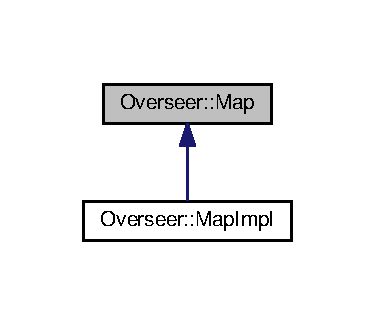
\includegraphics[width=180pt]{classOverseer_1_1Map__inherit__graph}
\end{center}
\end{figure}
\subsection*{Public Member Functions}
\begin{DoxyCompactItemize}
\item 
\hyperlink{classOverseer_1_1Map_a4f7eabe216b39eb4a63a8d0b4f8abf60}{Map} (sc2\+::\+Agent $\ast$bot)
\begin{DoxyCompactList}\small\item\em constructor. \end{DoxyCompactList}\item 
size\+\_\+t \hyperlink{classOverseer_1_1Map_a9993be7938014be6b9d66ffb0475a311}{get\+Height} () const 
\item 
size\+\_\+t \hyperlink{classOverseer_1_1Map_a803fae03c7ba59500f55c05dbc269c34}{get\+Width} () const 
\begin{DoxyCompactList}\small\item\em Gets the map width. \end{DoxyCompactList}\item 
std\+::vector$<$ std\+::shared\+\_\+ptr$<$ \hyperlink{classOverseer_1_1Region}{Region} $>$ $>$ \hyperlink{classOverseer_1_1Map_a90e9f9fd99091c142c4f07c5dc2ae7a3}{get\+Regions} ()
\begin{DoxyCompactList}\small\item\em Gets all the regions found. \end{DoxyCompactList}\item 
\hyperlink{classOverseer_1_1Region}{Region} $\ast$ \hyperlink{classOverseer_1_1Map_a419096dd4589e51c22b12018b8d9cbc1}{get\+Region} (size\+\_\+t id)
\begin{DoxyCompactList}\small\item\em Get a specific region. \end{DoxyCompactList}\item 
const \hyperlink{classOverseer_1_1Region}{Region} $\ast$ \hyperlink{classOverseer_1_1Map_ad49a674353cdf1fdda3aadc929fdbce0}{get\+Nearest\+Region} (sc2\+::\+Point2D pos)
\begin{DoxyCompactList}\small\item\em Gets closest region. \end{DoxyCompactList}\item 
void \hyperlink{classOverseer_1_1Map_afb26aba6abeaa039ae83b40c8235dee9}{add\+Tile} (sc2\+::\+Point2D \&pos, std\+::shared\+\_\+ptr$<$ \hyperlink{classOverseer_1_1Tile}{Tile} $>$ tile)
\begin{DoxyCompactList}\small\item\em Apends a tile to container. \end{DoxyCompactList}\item 
bool \hyperlink{classOverseer_1_1Map_a0cd63b3a16beab9b4cf01aa1b6adad8f}{Valid} (sc2\+::\+Point2D pos) const 
\begin{DoxyCompactList}\small\item\em Check if a position is on map. \end{DoxyCompactList}\item 
Tile\+Position \hyperlink{classOverseer_1_1Map_aebebc1ac43ea86747ebc38f2ee0d821d}{get\+Closest\+Tile\+Position} (sc2\+::\+Point2D pos)
\begin{DoxyCompactList}\small\item\em Get the closest tile position. \end{DoxyCompactList}\item 
void \hyperlink{classOverseer_1_1Map_afa19b5f826a5a4d37258e000bfa646a9}{add\+Region} (\hyperlink{classOverseer_1_1Region}{Region} region)
\begin{DoxyCompactList}\small\item\em Apends a region to the container. \end{DoxyCompactList}\item 
std\+::shared\+\_\+ptr$<$ \hyperlink{classOverseer_1_1Tile}{Tile} $>$ \hyperlink{classOverseer_1_1Map_a7df832c0a80c21cd79a18df2158f3989}{Get\+Tile} (sc2\+::\+Point2D pos)
\begin{DoxyCompactList}\small\item\em Gets a tile based on the position. \end{DoxyCompactList}\item 
size\+\_\+t \hyperlink{classOverseer_1_1Map_a29777413d8ac109aeb6f974a7b2fc25c}{size} ()
\begin{DoxyCompactList}\small\item\em Gets the size of the tile position container. \end{DoxyCompactList}\item 
Tile\+Position\+Container \hyperlink{classOverseer_1_1Map_a9e3000cfd9170cc7f6a70988fccd3af9}{get\+Tile\+Positions} ()
\begin{DoxyCompactList}\small\item\em Get all tile positions. \end{DoxyCompactList}\item 
void \hyperlink{classOverseer_1_1Map_a5fe859c4edbfc92971ad2ad38d69ff90}{set\+Bot} (sc2\+::\+Agent $\ast$bot)
\begin{DoxyCompactList}\small\item\em set the bot into overseer \end{DoxyCompactList}\item 
std\+::vector$<$ std\+::shared\+\_\+ptr$<$ Tile\+Position $>$ $>$ \hyperlink{classOverseer_1_1Map_a25596fe2da226652be51c7f80b28e28d}{get\+Frontier\+Positions} ()
\begin{DoxyCompactList}\small\item\em Get tiles that is between two regions. \end{DoxyCompactList}\item 
Raw\+Frontier \hyperlink{classOverseer_1_1Map_a7123e4389358218ad74ebce58680b6d2}{get\+Raw\+Frontier} ()
\begin{DoxyCompactList}\small\item\em region pair and frontier map. \end{DoxyCompactList}\end{DoxyCompactItemize}
\subsection*{Protected Member Functions}
\begin{DoxyCompactItemize}
\item 
std\+::pair$<$ size\+\_\+t, size\+\_\+t $>$ {\bfseries find\+Neighboring\+Regions} (std\+::shared\+\_\+ptr$<$ Tile\+Position $>$ tile\+Position)\hypertarget{classOverseer_1_1Map_aa27d53a051f421b9ea93e217b0313359}{}\label{classOverseer_1_1Map_aa27d53a051f421b9ea93e217b0313359}

\end{DoxyCompactItemize}
\subsection*{Protected Attributes}
\begin{DoxyCompactItemize}
\item 
sc2\+::\+Agent $\ast$ {\bfseries m\+\_\+bot}\hypertarget{classOverseer_1_1Map_a334ebcf2176817b4754911930dc5164e}{}\label{classOverseer_1_1Map_a334ebcf2176817b4754911930dc5164e}

\item 
Unit\+Position\+Container {\bfseries m\+\_\+unit\+Positions}\hypertarget{classOverseer_1_1Map_ac1e5514d3ddcfc418d5d1d7dac9e5213}{}\label{classOverseer_1_1Map_ac1e5514d3ddcfc418d5d1d7dac9e5213}

\item 
Tile\+Position\+Container {\bfseries m\+\_\+tile\+Positions}\hypertarget{classOverseer_1_1Map_ab2053a78e25fe4f3198ca63e0512ed69}{}\label{classOverseer_1_1Map_ab2053a78e25fe4f3198ca63e0512ed69}

\item 
std\+::vector$<$ std\+::shared\+\_\+ptr$<$ Tile\+Position $>$ $>$ {\bfseries m\+\_\+buildable\+Tiles}\hypertarget{classOverseer_1_1Map_a065b5150f280192f1447a9710b31b8ae}{}\label{classOverseer_1_1Map_a065b5150f280192f1447a9710b31b8ae}

\item 
Region\+Map {\bfseries m\+\_\+regions}\hypertarget{classOverseer_1_1Map_a450b4ef1ab3b6721011d76c20ab11af3}{}\label{classOverseer_1_1Map_a450b4ef1ab3b6721011d76c20ab11af3}

\item 
std\+::vector$<$ std\+::shared\+\_\+ptr$<$ Tile\+Position $>$ $>$ {\bfseries m\+\_\+frontier\+Positions}\hypertarget{classOverseer_1_1Map_a27bd6d65d0012db2c73b5c4bdf44fd6b}{}\label{classOverseer_1_1Map_a27bd6d65d0012db2c73b5c4bdf44fd6b}

\item 
Raw\+Frontier {\bfseries m\+\_\+raw\+Frontier}\hypertarget{classOverseer_1_1Map_a733ab6c5a8f43f4adb14159f10303e49}{}\label{classOverseer_1_1Map_a733ab6c5a8f43f4adb14159f10303e49}

\item 
sc2\+::\+Point2D {\bfseries m\+\_\+max\+Playable}\hypertarget{classOverseer_1_1Map_ac9b4cb658ce3dd3192244ea3f0c46f2a}{}\label{classOverseer_1_1Map_ac9b4cb658ce3dd3192244ea3f0c46f2a}

\item 
sc2\+::\+Point2D {\bfseries m\+\_\+min\+Playable}\hypertarget{classOverseer_1_1Map_a89e153ba6ab77c08f9e983db0f392a64}{}\label{classOverseer_1_1Map_a89e153ba6ab77c08f9e983db0f392a64}

\item 
sc2\+::\+Point2D {\bfseries m\+\_\+center\+Playable}\hypertarget{classOverseer_1_1Map_acbf0ee3e04e49c32fae495fbcc60702a}{}\label{classOverseer_1_1Map_acbf0ee3e04e49c32fae495fbcc60702a}

\item 
size\+\_\+t {\bfseries m\+\_\+width}\hypertarget{classOverseer_1_1Map_abc91b38cde7feb860dbe1f0be2d991bb}{}\label{classOverseer_1_1Map_abc91b38cde7feb860dbe1f0be2d991bb}

\item 
size\+\_\+t {\bfseries m\+\_\+height}\hypertarget{classOverseer_1_1Map_a686affcb69f23cbbd72f2be4f1061c90}{}\label{classOverseer_1_1Map_a686affcb69f23cbbd72f2be4f1061c90}

\end{DoxyCompactItemize}
\subsection*{Static Protected Attributes}
\begin{DoxyCompactItemize}
\item 
static std\+::unique\+\_\+ptr$<$ \hyperlink{classOverseer_1_1Map}{Map} $>$ {\bfseries m\+\_\+g\+Instance}\hypertarget{classOverseer_1_1Map_a7fac69d16e54ccfb3c477119f4a9ae69}{}\label{classOverseer_1_1Map_a7fac69d16e54ccfb3c477119f4a9ae69}

\end{DoxyCompactItemize}


\subsection{Detailed Description}
is the overseer map that holds the most \char`\"{}important\char`\"{} functionality for a outside user. 

\subsection{Constructor \& Destructor Documentation}
\index{Overseer\+::\+Map@{Overseer\+::\+Map}!Map@{Map}}
\index{Map@{Map}!Overseer\+::\+Map@{Overseer\+::\+Map}}
\subsubsection[{\texorpdfstring{Map(sc2\+::\+Agent $\ast$bot)}{Map(sc2::Agent *bot)}}]{\setlength{\rightskip}{0pt plus 5cm}Overseer\+::\+Map\+::\+Map (
\begin{DoxyParamCaption}
\item[{sc2\+::\+Agent $\ast$}]{bot}
\end{DoxyParamCaption}
)}\hypertarget{classOverseer_1_1Map_a4f7eabe216b39eb4a63a8d0b4f8abf60}{}\label{classOverseer_1_1Map_a4f7eabe216b39eb4a63a8d0b4f8abf60}


constructor. 


\begin{DoxyParams}{Parameters}
{\em bot} & The Starcraft II bot. \\
\hline
\end{DoxyParams}


\subsection{Member Function Documentation}
\index{Overseer\+::\+Map@{Overseer\+::\+Map}!add\+Region@{add\+Region}}
\index{add\+Region@{add\+Region}!Overseer\+::\+Map@{Overseer\+::\+Map}}
\subsubsection[{\texorpdfstring{add\+Region(\+Region region)}{addRegion(Region region)}}]{\setlength{\rightskip}{0pt plus 5cm}void Overseer\+::\+Map\+::add\+Region (
\begin{DoxyParamCaption}
\item[{{\bf Region}}]{region}
\end{DoxyParamCaption}
)}\hypertarget{classOverseer_1_1Map_afa19b5f826a5a4d37258e000bfa646a9}{}\label{classOverseer_1_1Map_afa19b5f826a5a4d37258e000bfa646a9}


Apends a region to the container. 


\begin{DoxyParams}{Parameters}
{\em region} & The \hyperlink{classOverseer_1_1Region}{Region} to apend. \\
\hline
\end{DoxyParams}
\index{Overseer\+::\+Map@{Overseer\+::\+Map}!add\+Tile@{add\+Tile}}
\index{add\+Tile@{add\+Tile}!Overseer\+::\+Map@{Overseer\+::\+Map}}
\subsubsection[{\texorpdfstring{add\+Tile(sc2\+::\+Point2\+D \&pos, std\+::shared\+\_\+ptr$<$ Tile $>$ tile)}{addTile(sc2::Point2D &pos, std::shared_ptr< Tile > tile)}}]{\setlength{\rightskip}{0pt plus 5cm}void Overseer\+::\+Map\+::add\+Tile (
\begin{DoxyParamCaption}
\item[{sc2\+::\+Point2D \&}]{pos, }
\item[{std\+::shared\+\_\+ptr$<$ {\bf Tile} $>$}]{tile}
\end{DoxyParamCaption}
)}\hypertarget{classOverseer_1_1Map_afb26aba6abeaa039ae83b40c8235dee9}{}\label{classOverseer_1_1Map_afb26aba6abeaa039ae83b40c8235dee9}


Apends a tile to container. 


\begin{DoxyParams}{Parameters}
{\em pos} & The tile position. \\
\hline
{\em tile} & The tile to add. \\
\hline
\end{DoxyParams}
\index{Overseer\+::\+Map@{Overseer\+::\+Map}!get\+Closest\+Tile\+Position@{get\+Closest\+Tile\+Position}}
\index{get\+Closest\+Tile\+Position@{get\+Closest\+Tile\+Position}!Overseer\+::\+Map@{Overseer\+::\+Map}}
\subsubsection[{\texorpdfstring{get\+Closest\+Tile\+Position(sc2\+::\+Point2\+D pos)}{getClosestTilePosition(sc2::Point2D pos)}}]{\setlength{\rightskip}{0pt plus 5cm}Tile\+Position Overseer\+::\+Map\+::get\+Closest\+Tile\+Position (
\begin{DoxyParamCaption}
\item[{sc2\+::\+Point2D}]{pos}
\end{DoxyParamCaption}
)}\hypertarget{classOverseer_1_1Map_aebebc1ac43ea86747ebc38f2ee0d821d}{}\label{classOverseer_1_1Map_aebebc1ac43ea86747ebc38f2ee0d821d}


Get the closest tile position. 


\begin{DoxyParams}{Parameters}
{\em pos} & of the tile position to find. \\
\hline
\end{DoxyParams}
\begin{DoxyReturn}{Returns}
the found tile position. 
\end{DoxyReturn}
\index{Overseer\+::\+Map@{Overseer\+::\+Map}!get\+Frontier\+Positions@{get\+Frontier\+Positions}}
\index{get\+Frontier\+Positions@{get\+Frontier\+Positions}!Overseer\+::\+Map@{Overseer\+::\+Map}}
\subsubsection[{\texorpdfstring{get\+Frontier\+Positions()}{getFrontierPositions()}}]{\setlength{\rightskip}{0pt plus 5cm}std\+::vector$<$ std\+::shared\+\_\+ptr$<$ Tile\+Position $>$ $>$ Overseer\+::\+Map\+::get\+Frontier\+Positions (
\begin{DoxyParamCaption}
{}
\end{DoxyParamCaption}
)}\hypertarget{classOverseer_1_1Map_a25596fe2da226652be51c7f80b28e28d}{}\label{classOverseer_1_1Map_a25596fe2da226652be51c7f80b28e28d}


Get tiles that is between two regions. 

\begin{DoxyReturn}{Returns}
vector with tile position pointers. 
\end{DoxyReturn}
\index{Overseer\+::\+Map@{Overseer\+::\+Map}!get\+Height@{get\+Height}}
\index{get\+Height@{get\+Height}!Overseer\+::\+Map@{Overseer\+::\+Map}}
\subsubsection[{\texorpdfstring{get\+Height() const }{getHeight() const }}]{\setlength{\rightskip}{0pt plus 5cm}size\+\_\+t Overseer\+::\+Map\+::get\+Height (
\begin{DoxyParamCaption}
{}
\end{DoxyParamCaption}
) const}\hypertarget{classOverseer_1_1Map_a9993be7938014be6b9d66ffb0475a311}{}\label{classOverseer_1_1Map_a9993be7938014be6b9d66ffb0475a311}
Gets the map height.

\begin{DoxyReturn}{Returns}
the height. 
\end{DoxyReturn}
\index{Overseer\+::\+Map@{Overseer\+::\+Map}!get\+Nearest\+Region@{get\+Nearest\+Region}}
\index{get\+Nearest\+Region@{get\+Nearest\+Region}!Overseer\+::\+Map@{Overseer\+::\+Map}}
\subsubsection[{\texorpdfstring{get\+Nearest\+Region(sc2\+::\+Point2\+D pos)}{getNearestRegion(sc2::Point2D pos)}}]{\setlength{\rightskip}{0pt plus 5cm}const {\bf Region} $\ast$ Overseer\+::\+Map\+::get\+Nearest\+Region (
\begin{DoxyParamCaption}
\item[{sc2\+::\+Point2D}]{pos}
\end{DoxyParamCaption}
)}\hypertarget{classOverseer_1_1Map_ad49a674353cdf1fdda3aadc929fdbce0}{}\label{classOverseer_1_1Map_ad49a674353cdf1fdda3aadc929fdbce0}


Gets closest region. 


\begin{DoxyParams}{Parameters}
{\em pos} & Is the position point to find region from. \\
\hline
\end{DoxyParams}
\begin{DoxyReturn}{Returns}
pointer to the found region. 
\end{DoxyReturn}
\index{Overseer\+::\+Map@{Overseer\+::\+Map}!get\+Raw\+Frontier@{get\+Raw\+Frontier}}
\index{get\+Raw\+Frontier@{get\+Raw\+Frontier}!Overseer\+::\+Map@{Overseer\+::\+Map}}
\subsubsection[{\texorpdfstring{get\+Raw\+Frontier()}{getRawFrontier()}}]{\setlength{\rightskip}{0pt plus 5cm}Raw\+Frontier Overseer\+::\+Map\+::get\+Raw\+Frontier (
\begin{DoxyParamCaption}
{}
\end{DoxyParamCaption}
)}\hypertarget{classOverseer_1_1Map_a7123e4389358218ad74ebce58680b6d2}{}\label{classOverseer_1_1Map_a7123e4389358218ad74ebce58680b6d2}


region pair and frontier map. 

\begin{DoxyReturn}{Returns}
vector of rawfrontier. 
\end{DoxyReturn}
\index{Overseer\+::\+Map@{Overseer\+::\+Map}!get\+Region@{get\+Region}}
\index{get\+Region@{get\+Region}!Overseer\+::\+Map@{Overseer\+::\+Map}}
\subsubsection[{\texorpdfstring{get\+Region(size\+\_\+t id)}{getRegion(size_t id)}}]{\setlength{\rightskip}{0pt plus 5cm}{\bf Region} $\ast$ Overseer\+::\+Map\+::get\+Region (
\begin{DoxyParamCaption}
\item[{size\+\_\+t}]{id}
\end{DoxyParamCaption}
)}\hypertarget{classOverseer_1_1Map_a419096dd4589e51c22b12018b8d9cbc1}{}\label{classOverseer_1_1Map_a419096dd4589e51c22b12018b8d9cbc1}


Get a specific region. 


\begin{DoxyParams}{Parameters}
{\em id} & The id of the specific region. \\
\hline
\end{DoxyParams}
\begin{DoxyReturn}{Returns}

\end{DoxyReturn}
\index{Overseer\+::\+Map@{Overseer\+::\+Map}!get\+Regions@{get\+Regions}}
\index{get\+Regions@{get\+Regions}!Overseer\+::\+Map@{Overseer\+::\+Map}}
\subsubsection[{\texorpdfstring{get\+Regions()}{getRegions()}}]{\setlength{\rightskip}{0pt plus 5cm}std\+::vector$<$ std\+::shared\+\_\+ptr$<$ {\bf Region} $>$ $>$ Overseer\+::\+Map\+::get\+Regions (
\begin{DoxyParamCaption}
{}
\end{DoxyParamCaption}
)}\hypertarget{classOverseer_1_1Map_a90e9f9fd99091c142c4f07c5dc2ae7a3}{}\label{classOverseer_1_1Map_a90e9f9fd99091c142c4f07c5dc2ae7a3}


Gets all the regions found. 

\begin{DoxyReturn}{Returns}
vector of region pointers. 
\end{DoxyReturn}
\index{Overseer\+::\+Map@{Overseer\+::\+Map}!Get\+Tile@{Get\+Tile}}
\index{Get\+Tile@{Get\+Tile}!Overseer\+::\+Map@{Overseer\+::\+Map}}
\subsubsection[{\texorpdfstring{Get\+Tile(sc2\+::\+Point2\+D pos)}{GetTile(sc2::Point2D pos)}}]{\setlength{\rightskip}{0pt plus 5cm}std\+::shared\+\_\+ptr$<$ {\bf Tile} $>$ Overseer\+::\+Map\+::\+Get\+Tile (
\begin{DoxyParamCaption}
\item[{sc2\+::\+Point2D}]{pos}
\end{DoxyParamCaption}
)}\hypertarget{classOverseer_1_1Map_a7df832c0a80c21cd79a18df2158f3989}{}\label{classOverseer_1_1Map_a7df832c0a80c21cd79a18df2158f3989}


Gets a tile based on the position. 


\begin{DoxyParams}{Parameters}
{\em pos} & The position of the tile. \\
\hline
\end{DoxyParams}
\begin{DoxyReturn}{Returns}
the found tile. 
\end{DoxyReturn}
\index{Overseer\+::\+Map@{Overseer\+::\+Map}!get\+Tile\+Positions@{get\+Tile\+Positions}}
\index{get\+Tile\+Positions@{get\+Tile\+Positions}!Overseer\+::\+Map@{Overseer\+::\+Map}}
\subsubsection[{\texorpdfstring{get\+Tile\+Positions()}{getTilePositions()}}]{\setlength{\rightskip}{0pt plus 5cm}Tile\+Position\+Container Overseer\+::\+Map\+::get\+Tile\+Positions (
\begin{DoxyParamCaption}
{}
\end{DoxyParamCaption}
)}\hypertarget{classOverseer_1_1Map_a9e3000cfd9170cc7f6a70988fccd3af9}{}\label{classOverseer_1_1Map_a9e3000cfd9170cc7f6a70988fccd3af9}


Get all tile positions. 

\begin{DoxyReturn}{Returns}
the tile position container. 
\end{DoxyReturn}
\index{Overseer\+::\+Map@{Overseer\+::\+Map}!get\+Width@{get\+Width}}
\index{get\+Width@{get\+Width}!Overseer\+::\+Map@{Overseer\+::\+Map}}
\subsubsection[{\texorpdfstring{get\+Width() const }{getWidth() const }}]{\setlength{\rightskip}{0pt plus 5cm}size\+\_\+t Overseer\+::\+Map\+::get\+Width (
\begin{DoxyParamCaption}
{}
\end{DoxyParamCaption}
) const}\hypertarget{classOverseer_1_1Map_a803fae03c7ba59500f55c05dbc269c34}{}\label{classOverseer_1_1Map_a803fae03c7ba59500f55c05dbc269c34}


Gets the map width. 

\begin{DoxyReturn}{Returns}
the width. 
\end{DoxyReturn}
\index{Overseer\+::\+Map@{Overseer\+::\+Map}!set\+Bot@{set\+Bot}}
\index{set\+Bot@{set\+Bot}!Overseer\+::\+Map@{Overseer\+::\+Map}}
\subsubsection[{\texorpdfstring{set\+Bot(sc2\+::\+Agent $\ast$bot)}{setBot(sc2::Agent *bot)}}]{\setlength{\rightskip}{0pt plus 5cm}void Overseer\+::\+Map\+::set\+Bot (
\begin{DoxyParamCaption}
\item[{sc2\+::\+Agent $\ast$}]{bot}
\end{DoxyParamCaption}
)}\hypertarget{classOverseer_1_1Map_a5fe859c4edbfc92971ad2ad38d69ff90}{}\label{classOverseer_1_1Map_a5fe859c4edbfc92971ad2ad38d69ff90}


set the bot into overseer 


\begin{DoxyParams}{Parameters}
{\em bot} & The bot witch overseer will use. \\
\hline
\end{DoxyParams}
\index{Overseer\+::\+Map@{Overseer\+::\+Map}!size@{size}}
\index{size@{size}!Overseer\+::\+Map@{Overseer\+::\+Map}}
\subsubsection[{\texorpdfstring{size()}{size()}}]{\setlength{\rightskip}{0pt plus 5cm}size\+\_\+t Overseer\+::\+Map\+::size (
\begin{DoxyParamCaption}
{}
\end{DoxyParamCaption}
)}\hypertarget{classOverseer_1_1Map_a29777413d8ac109aeb6f974a7b2fc25c}{}\label{classOverseer_1_1Map_a29777413d8ac109aeb6f974a7b2fc25c}


Gets the size of the tile position container. 

\begin{DoxyReturn}{Returns}
the size of container. 
\end{DoxyReturn}
\index{Overseer\+::\+Map@{Overseer\+::\+Map}!Valid@{Valid}}
\index{Valid@{Valid}!Overseer\+::\+Map@{Overseer\+::\+Map}}
\subsubsection[{\texorpdfstring{Valid(sc2\+::\+Point2\+D pos) const }{Valid(sc2::Point2D pos) const }}]{\setlength{\rightskip}{0pt plus 5cm}bool Overseer\+::\+Map\+::\+Valid (
\begin{DoxyParamCaption}
\item[{sc2\+::\+Point2D}]{pos}
\end{DoxyParamCaption}
) const}\hypertarget{classOverseer_1_1Map_a0cd63b3a16beab9b4cf01aa1b6adad8f}{}\label{classOverseer_1_1Map_a0cd63b3a16beab9b4cf01aa1b6adad8f}


Check if a position is on map. 

\begin{DoxyReturn}{Returns}
True if position is within the map, false otherwise. 
\end{DoxyReturn}


The documentation for this class was generated from the following files\+:\begin{DoxyCompactItemize}
\item 
/home/mejan/src/commandcenter/src/\+Overseer/src/Map.\+h\item 
/home/mejan/src/commandcenter/src/\+Overseer/src/Map.\+cpp\end{DoxyCompactItemize}

\hypertarget{classOverseer_1_1MapImpl}{}\section{Overseer\+:\+:Map\+Impl Class Reference}
\label{classOverseer_1_1MapImpl}\index{Overseer\+::\+Map\+Impl@{Overseer\+::\+Map\+Impl}}


The interface towards the map.  




{\ttfamily \#include \char`\"{}Map\+Impl.\+h\char`\"{}}



Inheritance diagram for Overseer\+:\+:Map\+Impl\+:
% FIG 0


Collaboration diagram for Overseer\+:\+:Map\+Impl\+:
% FIG 1
\subsection*{Public Member Functions}
\begin{DoxyCompactItemize}
\item 
\hyperlink{classOverseer_1_1MapImpl_a9c30887c6f342971fabd54d23b36a765}{Map\+Impl} (sc2\+::\+Agent $\ast$bot)
\begin{DoxyCompactList}\small\item\em constructor which adds the bot for temp control of map. \end{DoxyCompactList}\item 
void \hyperlink{classOverseer_1_1MapImpl_a5ec5b37d1ae07732a99845bfbbfce016}{Initialize} ()\hypertarget{classOverseer_1_1MapImpl_a5ec5b37d1ae07732a99845bfbbfce016}{}\label{classOverseer_1_1MapImpl_a5ec5b37d1ae07732a99845bfbbfce016}

\begin{DoxyCompactList}\small\item\em Initialize overseer, should be done after the map been loaded. \end{DoxyCompactList}\item 
\hyperlink{classOverseer_1_1Graph}{Graph} \hyperlink{classOverseer_1_1MapImpl_abedbb01faa88ff9bd3f8cd2dbec0dead}{get\+Graph} ()\hypertarget{classOverseer_1_1MapImpl_abedbb01faa88ff9bd3f8cd2dbec0dead}{}\label{classOverseer_1_1MapImpl_abedbb01faa88ff9bd3f8cd2dbec0dead}

\begin{DoxyCompactList}\small\item\em get the graph representation of the map. \end{DoxyCompactList}\end{DoxyCompactItemize}
\subsection*{Additional Inherited Members}


\subsection{Detailed Description}
The interface towards the map. 

\subsection{Constructor \& Destructor Documentation}
\index{Overseer\+::\+Map\+Impl@{Overseer\+::\+Map\+Impl}!Map\+Impl@{Map\+Impl}}
\index{Map\+Impl@{Map\+Impl}!Overseer\+::\+Map\+Impl@{Overseer\+::\+Map\+Impl}}
\subsubsection[{\texorpdfstring{Map\+Impl(sc2\+::\+Agent $\ast$bot)}{MapImpl(sc2::Agent *bot)}}]{\setlength{\rightskip}{0pt plus 5cm}Overseer\+::\+Map\+Impl\+::\+Map\+Impl (
\begin{DoxyParamCaption}
\item[{sc2\+::\+Agent $\ast$}]{bot}
\end{DoxyParamCaption}
)}\hypertarget{classOverseer_1_1MapImpl_a9c30887c6f342971fabd54d23b36a765}{}\label{classOverseer_1_1MapImpl_a9c30887c6f342971fabd54d23b36a765}


constructor which adds the bot for temp control of map. 


\begin{DoxyParams}{Parameters}
{\em bot} & Is the starcraft II bot currently run. \\
\hline
\end{DoxyParams}


The documentation for this class was generated from the following files\+:\begin{DoxyCompactItemize}
\item 
src/Map\+Impl.\+h\item 
src/Map\+Impl.\+cpp\end{DoxyCompactItemize}

\hypertarget{structOverseer_1_1NeutralImpl}{}\section{Overseer\+:\+:Neutral\+Impl Struct Reference}
\label{structOverseer_1_1NeutralImpl}\index{Overseer\+::\+Neutral\+Impl@{Overseer\+::\+Neutral\+Impl}}


Used to find neutral objects on the map.  


\subsection*{Public Member Functions}
\begin{DoxyCompactItemize}
\item 
\hyperlink{structOverseer_1_1NeutralImpl_a2ef6e7f65f2c6de6bc6beda0f020ba62}{Neutral\+Impl} (const sc2\+::\+Observation\+Interface $\ast$obs)
\begin{DoxyCompactList}\small\item\em Constructor sets all neutral positions to a map. \end{DoxyCompactList}\item 
bool \hyperlink{structOverseer_1_1NeutralImpl_a6bb0b123b5db8ab4285715d71a4d7e5b}{is\+Mineral} (sc2\+::\+Point2D \&pos)
\begin{DoxyCompactList}\small\item\em Check if a point is a mineral or not. \end{DoxyCompactList}\item 
bool \hyperlink{structOverseer_1_1NeutralImpl_a803959fe80b2b6bb14444a639b89acd5}{is\+Gas} (sc2\+::\+Point2D \&pos)
\begin{DoxyCompactList}\small\item\em Check if a point is a geyser or not. \end{DoxyCompactList}\item 
bool \hyperlink{structOverseer_1_1NeutralImpl_af8393ea00dad811b9132403e73d68f83}{is\+Destructible} (sc2\+::\+Point2D \&pos)
\begin{DoxyCompactList}\small\item\em Check if a point is a destructable object or not. \end{DoxyCompactList}\item 
bool \hyperlink{structOverseer_1_1NeutralImpl_a8e874807b118a287811311a033c98dc2}{is\+Naga\+Tower} (sc2\+::\+Point2D \&pos)
\begin{DoxyCompactList}\small\item\em Check if a point is a Xelnaga tower or not. \end{DoxyCompactList}\end{DoxyCompactItemize}


\subsection{Detailed Description}
Used to find neutral objects on the map. 

\subsection{Constructor \& Destructor Documentation}
\mbox{\Hypertarget{structOverseer_1_1NeutralImpl_a2ef6e7f65f2c6de6bc6beda0f020ba62}\label{structOverseer_1_1NeutralImpl_a2ef6e7f65f2c6de6bc6beda0f020ba62}} 
\index{Overseer\+::\+Neutral\+Impl@{Overseer\+::\+Neutral\+Impl}!Neutral\+Impl@{Neutral\+Impl}}
\index{Neutral\+Impl@{Neutral\+Impl}!Overseer\+::\+Neutral\+Impl@{Overseer\+::\+Neutral\+Impl}}
\subsubsection{\texorpdfstring{Neutral\+Impl()}{NeutralImpl()}}
{\footnotesize\ttfamily Overseer\+::\+Neutral\+Impl\+::\+Neutral\+Impl (\begin{DoxyParamCaption}\item[{const sc2\+::\+Observation\+Interface $\ast$}]{obs }\end{DoxyParamCaption})}



Constructor sets all neutral positions to a map. 


\begin{DoxyParams}{Parameters}
{\em obs} & used to discover neutrals on the map. \\
\hline
\end{DoxyParams}


\subsection{Member Function Documentation}
\mbox{\Hypertarget{structOverseer_1_1NeutralImpl_af8393ea00dad811b9132403e73d68f83}\label{structOverseer_1_1NeutralImpl_af8393ea00dad811b9132403e73d68f83}} 
\index{Overseer\+::\+Neutral\+Impl@{Overseer\+::\+Neutral\+Impl}!is\+Destructible@{is\+Destructible}}
\index{is\+Destructible@{is\+Destructible}!Overseer\+::\+Neutral\+Impl@{Overseer\+::\+Neutral\+Impl}}
\subsubsection{\texorpdfstring{is\+Destructible()}{isDestructible()}}
{\footnotesize\ttfamily bool Overseer\+::\+Neutral\+Impl\+::is\+Destructible (\begin{DoxyParamCaption}\item[{sc2\+::\+Point2D \&}]{pos }\end{DoxyParamCaption})}



Check if a point is a destructable object or not. 


\begin{DoxyParams}{Parameters}
{\em pos} & the point to check. \\
\hline
\end{DoxyParams}
\begin{DoxyReturn}{Returns}
true if it is destructable object, otherwise false. 
\end{DoxyReturn}
\mbox{\Hypertarget{structOverseer_1_1NeutralImpl_a803959fe80b2b6bb14444a639b89acd5}\label{structOverseer_1_1NeutralImpl_a803959fe80b2b6bb14444a639b89acd5}} 
\index{Overseer\+::\+Neutral\+Impl@{Overseer\+::\+Neutral\+Impl}!is\+Gas@{is\+Gas}}
\index{is\+Gas@{is\+Gas}!Overseer\+::\+Neutral\+Impl@{Overseer\+::\+Neutral\+Impl}}
\subsubsection{\texorpdfstring{is\+Gas()}{isGas()}}
{\footnotesize\ttfamily bool Overseer\+::\+Neutral\+Impl\+::is\+Gas (\begin{DoxyParamCaption}\item[{sc2\+::\+Point2D \&}]{pos }\end{DoxyParamCaption})}



Check if a point is a geyser or not. 


\begin{DoxyParams}{Parameters}
{\em pos} & the point to check. \\
\hline
\end{DoxyParams}
\begin{DoxyReturn}{Returns}
true if it is geyser, otherwise false. 
\end{DoxyReturn}
\mbox{\Hypertarget{structOverseer_1_1NeutralImpl_a6bb0b123b5db8ab4285715d71a4d7e5b}\label{structOverseer_1_1NeutralImpl_a6bb0b123b5db8ab4285715d71a4d7e5b}} 
\index{Overseer\+::\+Neutral\+Impl@{Overseer\+::\+Neutral\+Impl}!is\+Mineral@{is\+Mineral}}
\index{is\+Mineral@{is\+Mineral}!Overseer\+::\+Neutral\+Impl@{Overseer\+::\+Neutral\+Impl}}
\subsubsection{\texorpdfstring{is\+Mineral()}{isMineral()}}
{\footnotesize\ttfamily bool Overseer\+::\+Neutral\+Impl\+::is\+Mineral (\begin{DoxyParamCaption}\item[{sc2\+::\+Point2D \&}]{pos }\end{DoxyParamCaption})}



Check if a point is a mineral or not. 


\begin{DoxyParams}{Parameters}
{\em pos} & the point to check. \\
\hline
\end{DoxyParams}
\begin{DoxyReturn}{Returns}
true if point is mineral, otherwise false. 
\end{DoxyReturn}
\mbox{\Hypertarget{structOverseer_1_1NeutralImpl_a8e874807b118a287811311a033c98dc2}\label{structOverseer_1_1NeutralImpl_a8e874807b118a287811311a033c98dc2}} 
\index{Overseer\+::\+Neutral\+Impl@{Overseer\+::\+Neutral\+Impl}!is\+Naga\+Tower@{is\+Naga\+Tower}}
\index{is\+Naga\+Tower@{is\+Naga\+Tower}!Overseer\+::\+Neutral\+Impl@{Overseer\+::\+Neutral\+Impl}}
\subsubsection{\texorpdfstring{is\+Naga\+Tower()}{isNagaTower()}}
{\footnotesize\ttfamily bool Overseer\+::\+Neutral\+Impl\+::is\+Naga\+Tower (\begin{DoxyParamCaption}\item[{sc2\+::\+Point2D \&}]{pos }\end{DoxyParamCaption})}



Check if a point is a Xelnaga tower or not. 


\begin{DoxyParams}{Parameters}
{\em pos} & the point to check. \\
\hline
\end{DoxyParams}
\begin{DoxyReturn}{Returns}
true if it is Xelnaga tower, otherwise false. 
\end{DoxyReturn}


The documentation for this struct was generated from the following files\+:\begin{DoxyCompactItemize}
\item 
src/Neutral\+Set\+Obj.\+h\item 
src/Neutral\+Set\+Obj.\+cpp\end{DoxyCompactItemize}

\hypertarget{structOverseer_1_1accessors_1_1point2d__accessor}{}\section{Overseer\+:\+:accessors\+:\+:point2d\+\_\+accessor Struct Reference}
\label{structOverseer_1_1accessors_1_1point2d__accessor}\index{Overseer\+::accessors\+::point2d\+\_\+accessor@{Overseer\+::accessors\+::point2d\+\_\+accessor}}
\subsection*{Public Member Functions}
\begin{DoxyCompactItemize}
\item 
\mbox{\Hypertarget{structOverseer_1_1accessors_1_1point2d__accessor_aa698247566da77479df81656067ec995}\label{structOverseer_1_1accessors_1_1point2d__accessor_aa698247566da77479df81656067ec995}} 
int {\bfseries operator()} (spatial\+::dimension\+\_\+type dim, const sc2\+::\+Point2D p) const
\end{DoxyCompactItemize}


The documentation for this struct was generated from the following file\+:\begin{DoxyCompactItemize}
\item 
src/Definitions.\+h\end{DoxyCompactItemize}

\hypertarget{classOverseer_1_1Region}{}\section{Overseer\+:\+:Region Class Reference}
\label{classOverseer_1_1Region}\index{Overseer\+::\+Region@{Overseer\+::\+Region}}


A region handler.  




{\ttfamily \#include \char`\"{}Region.\+h\char`\"{}}

\subsection*{Public Member Functions}
\begin{DoxyCompactItemize}
\item 
\mbox{\Hypertarget{classOverseer_1_1Region_af241efba7a6115b1b1526924ad114ec1}\label{classOverseer_1_1Region_af241efba7a6115b1b1526924ad114ec1}} 
\hyperlink{classOverseer_1_1Region_af241efba7a6115b1b1526924ad114ec1}{Region} ()
\begin{DoxyCompactList}\small\item\em default constructor. \end{DoxyCompactList}\item 
\hyperlink{classOverseer_1_1Region_a8de3309b915589c86745a73c157d4a9f}{Region} (size\+\_\+t region\+Id, std\+::shared\+\_\+ptr$<$ Tile\+Position $>$ tile\+Position)
\begin{DoxyCompactList}\small\item\em constructor. \end{DoxyCompactList}\item 
size\+\_\+t \hyperlink{classOverseer_1_1Region_ae0c44ec954897475619ed302cf5a36e4}{get\+Area} () const
\begin{DoxyCompactList}\small\item\em Gets the number of points within the region, which corresponds to it\textquotesingle{}s area. \end{DoxyCompactList}\item 
const std\+::vector$<$ Unit\+Position $>$ \hyperlink{classOverseer_1_1Region_a9ac3f900c0b0b260ded354769337149d}{get\+Neutral\+Unit\+Positions} ()
\begin{DoxyCompactList}\small\item\em Returns the edges of the region. \end{DoxyCompactList}\item 
size\+\_\+t \hyperlink{classOverseer_1_1Region_aad3eddafae817b164847dafdf025d13c}{get\+Id} () const
\begin{DoxyCompactList}\small\item\em Get region id. \end{DoxyCompactList}\item 
void \hyperlink{classOverseer_1_1Region_a52fa1e6684d036d9f2761ec4cf85cd62}{set\+Id} (size\+\_\+t region\+Id)
\begin{DoxyCompactList}\small\item\em set the region id (I\+N\+T\+E\+R\+N\+AL U\+SE O\+N\+LY) \end{DoxyCompactList}\item 
std\+::vector$<$ Tile\+Position $>$ \hyperlink{classOverseer_1_1Region_a3977361e7b25ecc320a8a71af13c3f07}{get\+Tile\+Positions} () const
\begin{DoxyCompactList}\small\item\em Get the tile positions within the region. \end{DoxyCompactList}\item 
std\+::vector$<$ sc2\+::\+Point2D $>$ \hyperlink{classOverseer_1_1Region_a9e2a9eaeee365e31aa38528e929772d4}{get\+Points} () const
\begin{DoxyCompactList}\small\item\em Gets all mid points from all tiles within this region. \end{DoxyCompactList}\item 
void \hyperlink{classOverseer_1_1Region_aacbbc5db08289919979c40638b90ff7f}{add\+Tile\+Position} (std\+::shared\+\_\+ptr$<$ Tile\+Position $>$ tile\+Position)
\begin{DoxyCompactList}\small\item\em Add tile position to region. \end{DoxyCompactList}\item 
void \hyperlink{classOverseer_1_1Region_a95f03d39e96fdb038bfa8d55c3609896}{add\+Tile\+Position} (Tile\+Position \&tile\+Position)
\begin{DoxyCompactList}\small\item\em Add tile position to region. \end{DoxyCompactList}\item 
double \hyperlink{classOverseer_1_1Region_ac8816d6a083ad2a1fe153390b255ebfe}{get\+Largest\+Distance\+To\+Unpathable} () const
\begin{DoxyCompactList}\small\item\em get the longest path to a unpathable. \end{DoxyCompactList}\item 
sc2\+::\+Point2D \hyperlink{classOverseer_1_1Region_aabaca16412cb07744db2807121450c1e}{get\+Mid\+Point} () const
\begin{DoxyCompactList}\small\item\em Get the mid point of this region. \end{DoxyCompactList}\item 
void \hyperlink{classOverseer_1_1Region_ad532499817aecf45c88387a1a775a2fd}{merge} (\hyperlink{classOverseer_1_1Region}{Region} region)
\begin{DoxyCompactList}\small\item\em Merges two regions (I\+N\+T\+E\+R\+N\+AL U\+SE O\+N\+LY). \end{DoxyCompactList}\item 
\mbox{\Hypertarget{classOverseer_1_1Region_a945c843e2061f5de20cfaf7e45fa0568}\label{classOverseer_1_1Region_a945c843e2061f5de20cfaf7e45fa0568}} 
void \hyperlink{classOverseer_1_1Region_a945c843e2061f5de20cfaf7e45fa0568}{clear} ()
\begin{DoxyCompactList}\small\item\em clear this region of its tile positions (I\+N\+T\+E\+R\+N\+AL U\+SE O\+N\+LY). \end{DoxyCompactList}\end{DoxyCompactItemize}


\subsection{Detailed Description}
A region handler. 

\subsection{Constructor \& Destructor Documentation}
\mbox{\Hypertarget{classOverseer_1_1Region_a8de3309b915589c86745a73c157d4a9f}\label{classOverseer_1_1Region_a8de3309b915589c86745a73c157d4a9f}} 
\index{Overseer\+::\+Region@{Overseer\+::\+Region}!Region@{Region}}
\index{Region@{Region}!Overseer\+::\+Region@{Overseer\+::\+Region}}
\subsubsection{\texorpdfstring{Region()}{Region()}}
{\footnotesize\ttfamily Overseer\+::\+Region\+::\+Region (\begin{DoxyParamCaption}\item[{size\+\_\+t}]{region\+Id,  }\item[{std\+::shared\+\_\+ptr$<$ Tile\+Position $>$}]{tile\+Position }\end{DoxyParamCaption})}



constructor. 


\begin{DoxyParams}{Parameters}
{\em region\+Id} & The id a region \\
\hline
{\em tile\+Position} & A tileposition within the region. \\
\hline
\end{DoxyParams}


\subsection{Member Function Documentation}
\mbox{\Hypertarget{classOverseer_1_1Region_aacbbc5db08289919979c40638b90ff7f}\label{classOverseer_1_1Region_aacbbc5db08289919979c40638b90ff7f}} 
\index{Overseer\+::\+Region@{Overseer\+::\+Region}!add\+Tile\+Position@{add\+Tile\+Position}}
\index{add\+Tile\+Position@{add\+Tile\+Position}!Overseer\+::\+Region@{Overseer\+::\+Region}}
\subsubsection{\texorpdfstring{add\+Tile\+Position()}{addTilePosition()}\hspace{0.1cm}{\footnotesize\ttfamily [1/2]}}
{\footnotesize\ttfamily void Overseer\+::\+Region\+::add\+Tile\+Position (\begin{DoxyParamCaption}\item[{std\+::shared\+\_\+ptr$<$ Tile\+Position $>$}]{tile\+Position }\end{DoxyParamCaption})}



Add tile position to region. 


\begin{DoxyParams}{Parameters}
{\em the} & tile position to add. \\
\hline
\end{DoxyParams}
\mbox{\Hypertarget{classOverseer_1_1Region_a95f03d39e96fdb038bfa8d55c3609896}\label{classOverseer_1_1Region_a95f03d39e96fdb038bfa8d55c3609896}} 
\index{Overseer\+::\+Region@{Overseer\+::\+Region}!add\+Tile\+Position@{add\+Tile\+Position}}
\index{add\+Tile\+Position@{add\+Tile\+Position}!Overseer\+::\+Region@{Overseer\+::\+Region}}
\subsubsection{\texorpdfstring{add\+Tile\+Position()}{addTilePosition()}\hspace{0.1cm}{\footnotesize\ttfamily [2/2]}}
{\footnotesize\ttfamily void Overseer\+::\+Region\+::add\+Tile\+Position (\begin{DoxyParamCaption}\item[{Tile\+Position \&}]{tile\+Position }\end{DoxyParamCaption})}



Add tile position to region. 


\begin{DoxyParams}{Parameters}
{\em the} & tile position to add. \\
\hline
\end{DoxyParams}
\mbox{\Hypertarget{classOverseer_1_1Region_ae0c44ec954897475619ed302cf5a36e4}\label{classOverseer_1_1Region_ae0c44ec954897475619ed302cf5a36e4}} 
\index{Overseer\+::\+Region@{Overseer\+::\+Region}!get\+Area@{get\+Area}}
\index{get\+Area@{get\+Area}!Overseer\+::\+Region@{Overseer\+::\+Region}}
\subsubsection{\texorpdfstring{get\+Area()}{getArea()}}
{\footnotesize\ttfamily size\+\_\+t Overseer\+::\+Region\+::get\+Area (\begin{DoxyParamCaption}{ }\end{DoxyParamCaption}) const}



Gets the number of points within the region, which corresponds to it\textquotesingle{}s area. 

\begin{DoxyReturn}{Returns}
The number of tile positiions within the region. 
\end{DoxyReturn}
\mbox{\Hypertarget{classOverseer_1_1Region_aad3eddafae817b164847dafdf025d13c}\label{classOverseer_1_1Region_aad3eddafae817b164847dafdf025d13c}} 
\index{Overseer\+::\+Region@{Overseer\+::\+Region}!get\+Id@{get\+Id}}
\index{get\+Id@{get\+Id}!Overseer\+::\+Region@{Overseer\+::\+Region}}
\subsubsection{\texorpdfstring{get\+Id()}{getId()}}
{\footnotesize\ttfamily size\+\_\+t Overseer\+::\+Region\+::get\+Id (\begin{DoxyParamCaption}{ }\end{DoxyParamCaption}) const}



Get region id. 

\begin{DoxyReturn}{Returns}
This region id 
\end{DoxyReturn}
\mbox{\Hypertarget{classOverseer_1_1Region_ac8816d6a083ad2a1fe153390b255ebfe}\label{classOverseer_1_1Region_ac8816d6a083ad2a1fe153390b255ebfe}} 
\index{Overseer\+::\+Region@{Overseer\+::\+Region}!get\+Largest\+Distance\+To\+Unpathable@{get\+Largest\+Distance\+To\+Unpathable}}
\index{get\+Largest\+Distance\+To\+Unpathable@{get\+Largest\+Distance\+To\+Unpathable}!Overseer\+::\+Region@{Overseer\+::\+Region}}
\subsubsection{\texorpdfstring{get\+Largest\+Distance\+To\+Unpathable()}{getLargestDistanceToUnpathable()}}
{\footnotesize\ttfamily double Overseer\+::\+Region\+::get\+Largest\+Distance\+To\+Unpathable (\begin{DoxyParamCaption}{ }\end{DoxyParamCaption}) const}



get the longest path to a unpathable. 

\begin{DoxyReturn}{Returns}
the path. 
\end{DoxyReturn}
\mbox{\Hypertarget{classOverseer_1_1Region_aabaca16412cb07744db2807121450c1e}\label{classOverseer_1_1Region_aabaca16412cb07744db2807121450c1e}} 
\index{Overseer\+::\+Region@{Overseer\+::\+Region}!get\+Mid\+Point@{get\+Mid\+Point}}
\index{get\+Mid\+Point@{get\+Mid\+Point}!Overseer\+::\+Region@{Overseer\+::\+Region}}
\subsubsection{\texorpdfstring{get\+Mid\+Point()}{getMidPoint()}}
{\footnotesize\ttfamily sc2\+::\+Point2D Overseer\+::\+Region\+::get\+Mid\+Point (\begin{DoxyParamCaption}{ }\end{DoxyParamCaption}) const}



Get the mid point of this region. 

\begin{DoxyReturn}{Returns}
region mid point 
\end{DoxyReturn}
\mbox{\Hypertarget{classOverseer_1_1Region_a9ac3f900c0b0b260ded354769337149d}\label{classOverseer_1_1Region_a9ac3f900c0b0b260ded354769337149d}} 
\index{Overseer\+::\+Region@{Overseer\+::\+Region}!get\+Neutral\+Unit\+Positions@{get\+Neutral\+Unit\+Positions}}
\index{get\+Neutral\+Unit\+Positions@{get\+Neutral\+Unit\+Positions}!Overseer\+::\+Region@{Overseer\+::\+Region}}
\subsubsection{\texorpdfstring{get\+Neutral\+Unit\+Positions()}{getNeutralUnitPositions()}}
{\footnotesize\ttfamily const std\+::vector$<$ Unit\+Position $>$ Overseer\+::\+Region\+::get\+Neutral\+Unit\+Positions (\begin{DoxyParamCaption}{ }\end{DoxyParamCaption})}



Returns the edges of the region. 

\begin{DoxyReturn}{Returns}
vector with edges. Returns the units and positions occupying the region

const vector with unit positions. 
\end{DoxyReturn}
\mbox{\Hypertarget{classOverseer_1_1Region_a9e2a9eaeee365e31aa38528e929772d4}\label{classOverseer_1_1Region_a9e2a9eaeee365e31aa38528e929772d4}} 
\index{Overseer\+::\+Region@{Overseer\+::\+Region}!get\+Points@{get\+Points}}
\index{get\+Points@{get\+Points}!Overseer\+::\+Region@{Overseer\+::\+Region}}
\subsubsection{\texorpdfstring{get\+Points()}{getPoints()}}
{\footnotesize\ttfamily std\+::vector$<$ sc2\+::\+Point2D $>$ Overseer\+::\+Region\+::get\+Points (\begin{DoxyParamCaption}{ }\end{DoxyParamCaption}) const}



Gets all mid points from all tiles within this region. 

\begin{DoxyReturn}{Returns}
vector the sc2\+::\+Point2D 
\end{DoxyReturn}
\mbox{\Hypertarget{classOverseer_1_1Region_a3977361e7b25ecc320a8a71af13c3f07}\label{classOverseer_1_1Region_a3977361e7b25ecc320a8a71af13c3f07}} 
\index{Overseer\+::\+Region@{Overseer\+::\+Region}!get\+Tile\+Positions@{get\+Tile\+Positions}}
\index{get\+Tile\+Positions@{get\+Tile\+Positions}!Overseer\+::\+Region@{Overseer\+::\+Region}}
\subsubsection{\texorpdfstring{get\+Tile\+Positions()}{getTilePositions()}}
{\footnotesize\ttfamily std\+::vector$<$ Tile\+Position $>$ Overseer\+::\+Region\+::get\+Tile\+Positions (\begin{DoxyParamCaption}{ }\end{DoxyParamCaption}) const}



Get the tile positions within the region. 

\begin{DoxyReturn}{Returns}
vector with tileposition. 
\end{DoxyReturn}
\mbox{\Hypertarget{classOverseer_1_1Region_ad532499817aecf45c88387a1a775a2fd}\label{classOverseer_1_1Region_ad532499817aecf45c88387a1a775a2fd}} 
\index{Overseer\+::\+Region@{Overseer\+::\+Region}!merge@{merge}}
\index{merge@{merge}!Overseer\+::\+Region@{Overseer\+::\+Region}}
\subsubsection{\texorpdfstring{merge()}{merge()}}
{\footnotesize\ttfamily void Overseer\+::\+Region\+::merge (\begin{DoxyParamCaption}\item[{\hyperlink{classOverseer_1_1Region}{Region}}]{region }\end{DoxyParamCaption})}



Merges two regions (I\+N\+T\+E\+R\+N\+AL U\+SE O\+N\+LY). 


\begin{DoxyParams}{Parameters}
{\em region} & The region to merge with T\+H\+IS region. \\
\hline
\end{DoxyParams}
\mbox{\Hypertarget{classOverseer_1_1Region_a52fa1e6684d036d9f2761ec4cf85cd62}\label{classOverseer_1_1Region_a52fa1e6684d036d9f2761ec4cf85cd62}} 
\index{Overseer\+::\+Region@{Overseer\+::\+Region}!set\+Id@{set\+Id}}
\index{set\+Id@{set\+Id}!Overseer\+::\+Region@{Overseer\+::\+Region}}
\subsubsection{\texorpdfstring{set\+Id()}{setId()}}
{\footnotesize\ttfamily void Overseer\+::\+Region\+::set\+Id (\begin{DoxyParamCaption}\item[{size\+\_\+t}]{region\+Id }\end{DoxyParamCaption})}



set the region id (I\+N\+T\+E\+R\+N\+AL U\+SE O\+N\+LY) 


\begin{DoxyParams}{Parameters}
{\em the} & id to set \\
\hline
\end{DoxyParams}


The documentation for this class was generated from the following files\+:\begin{DoxyCompactItemize}
\item 
src/Region.\+h\item 
src/Region.\+cpp\end{DoxyCompactItemize}

\hypertarget{classRegionEdge}{}\section{Region\+Edge Class Reference}
\label{classRegionEdge}\index{Region\+Edge@{Region\+Edge}}


Edge handliing for a region. --inprogress.  




{\ttfamily \#include \char`\"{}Region.\+h\char`\"{}}



\subsection{Detailed Description}
Edge handliing for a region. --inprogress. 

The documentation for this class was generated from the following file\+:\begin{DoxyCompactItemize}
\item 
src/Region.\+h\end{DoxyCompactItemize}

\hypertarget{classOverseer_1_1Tile}{}\section{Overseer\+:\+:Tile Class Reference}
\label{classOverseer_1_1Tile}\index{Overseer\+::\+Tile@{Overseer\+::\+Tile}}


A tile is area that has size 1x1 within S\+C\+II maps.  




{\ttfamily \#include \char`\"{}Tile.\+h\char`\"{}}

\subsection*{Public Member Functions}
\begin{DoxyCompactItemize}
\item 
Tile\+Terrain \hyperlink{classOverseer_1_1Tile_aeddd0f013514a193e8da23bdeafdd6b9}{get\+Tile\+Terrain} ()
\begin{DoxyCompactList}\small\item\em Says what type of terrain it is on this tile, see Tile\+Terrain for alteritives. \end{DoxyCompactList}\item 
float \hyperlink{classOverseer_1_1Tile_a22171679810a298d4119b997004d3e13}{get\+Terrain\+Height} ()
\begin{DoxyCompactList}\small\item\em Get the z-\/axis value for the tile. \end{DoxyCompactList}\item 
void \hyperlink{classOverseer_1_1Tile_a79f2aa12d9463e7e4bfc85b8bdddbc34}{set\+Terrain\+Height} (float height)
\begin{DoxyCompactList}\small\item\em Sets the z-\/axis value for the tile. \end{DoxyCompactList}\item 
void \hyperlink{classOverseer_1_1Tile_a22494032e2b92af9c4e4b375845fd80f}{set\+Tile\+Terrain} (Tile\+Terrain \&terrain)
\begin{DoxyCompactList}\small\item\em If there exist build or wall. \end{DoxyCompactList}\item 
void \hyperlink{classOverseer_1_1Tile_a5a3b3f84b703b2cd5a9ae56b60e77b4c}{set\+Dist\+Nearest\+Unpathable} (float dist)
\begin{DoxyCompactList}\small\item\em Set a distance to the nearest unpathable tile. \end{DoxyCompactList}\item 
float \hyperlink{classOverseer_1_1Tile_a120fd6da5041e8c60bb8d92caa111576}{get\+Dist\+Nearest\+Unpathable} () const
\begin{DoxyCompactList}\small\item\em Get the distance to nearest unpathable. \end{DoxyCompactList}\item 
void \hyperlink{classOverseer_1_1Tile_a8f0f9bc7bd55533a4df7cf2cafc08eaa}{set\+Region\+Id} (size\+\_\+t region\+Id)
\begin{DoxyCompactList}\small\item\em Set the region id this tile belong to. \end{DoxyCompactList}\item 
size\+\_\+t \hyperlink{classOverseer_1_1Tile_aa1fa9037029a36f50b3c13130813e825}{get\+Region\+Id} ()
\begin{DoxyCompactList}\small\item\em Get the region id this tile is in. \end{DoxyCompactList}\item 
\mbox{\Hypertarget{classOverseer_1_1Tile_ae2e7f85589e4963a0474b038cff3daa0}\label{classOverseer_1_1Tile_ae2e7f85589e4963a0474b038cff3daa0}} 
bool \hyperlink{classOverseer_1_1Tile_ae2e7f85589e4963a0474b038cff3daa0}{is\+Neutral} ()
\begin{DoxyCompactList}\small\item\em Check if the tile contain neutral unit, e.\+g. gas, miniral and destroable. \end{DoxyCompactList}\end{DoxyCompactItemize}


\subsection{Detailed Description}
A tile is area that has size 1x1 within S\+C\+II maps. 

\subsection{Member Function Documentation}
\mbox{\Hypertarget{classOverseer_1_1Tile_a120fd6da5041e8c60bb8d92caa111576}\label{classOverseer_1_1Tile_a120fd6da5041e8c60bb8d92caa111576}} 
\index{Overseer\+::\+Tile@{Overseer\+::\+Tile}!get\+Dist\+Nearest\+Unpathable@{get\+Dist\+Nearest\+Unpathable}}
\index{get\+Dist\+Nearest\+Unpathable@{get\+Dist\+Nearest\+Unpathable}!Overseer\+::\+Tile@{Overseer\+::\+Tile}}
\subsubsection{\texorpdfstring{get\+Dist\+Nearest\+Unpathable()}{getDistNearestUnpathable()}}
{\footnotesize\ttfamily float Overseer\+::\+Tile\+::get\+Dist\+Nearest\+Unpathable (\begin{DoxyParamCaption}{ }\end{DoxyParamCaption}) const}



Get the distance to nearest unpathable. 

\begin{DoxyReturn}{Returns}
distance. 
\end{DoxyReturn}
\mbox{\Hypertarget{classOverseer_1_1Tile_aa1fa9037029a36f50b3c13130813e825}\label{classOverseer_1_1Tile_aa1fa9037029a36f50b3c13130813e825}} 
\index{Overseer\+::\+Tile@{Overseer\+::\+Tile}!get\+Region\+Id@{get\+Region\+Id}}
\index{get\+Region\+Id@{get\+Region\+Id}!Overseer\+::\+Tile@{Overseer\+::\+Tile}}
\subsubsection{\texorpdfstring{get\+Region\+Id()}{getRegionId()}}
{\footnotesize\ttfamily size\+\_\+t Overseer\+::\+Tile\+::get\+Region\+Id (\begin{DoxyParamCaption}{ }\end{DoxyParamCaption})}



Get the region id this tile is in. 

\begin{DoxyReturn}{Returns}
regionid 
\end{DoxyReturn}
\mbox{\Hypertarget{classOverseer_1_1Tile_a22171679810a298d4119b997004d3e13}\label{classOverseer_1_1Tile_a22171679810a298d4119b997004d3e13}} 
\index{Overseer\+::\+Tile@{Overseer\+::\+Tile}!get\+Terrain\+Height@{get\+Terrain\+Height}}
\index{get\+Terrain\+Height@{get\+Terrain\+Height}!Overseer\+::\+Tile@{Overseer\+::\+Tile}}
\subsubsection{\texorpdfstring{get\+Terrain\+Height()}{getTerrainHeight()}}
{\footnotesize\ttfamily float Overseer\+::\+Tile\+::get\+Terrain\+Height (\begin{DoxyParamCaption}{ }\end{DoxyParamCaption})}



Get the z-\/axis value for the tile. 

\begin{DoxyReturn}{Returns}
z-\/axis value. 
\end{DoxyReturn}
\mbox{\Hypertarget{classOverseer_1_1Tile_aeddd0f013514a193e8da23bdeafdd6b9}\label{classOverseer_1_1Tile_aeddd0f013514a193e8da23bdeafdd6b9}} 
\index{Overseer\+::\+Tile@{Overseer\+::\+Tile}!get\+Tile\+Terrain@{get\+Tile\+Terrain}}
\index{get\+Tile\+Terrain@{get\+Tile\+Terrain}!Overseer\+::\+Tile@{Overseer\+::\+Tile}}
\subsubsection{\texorpdfstring{get\+Tile\+Terrain()}{getTileTerrain()}}
{\footnotesize\ttfamily Tile\+Terrain Overseer\+::\+Tile\+::get\+Tile\+Terrain (\begin{DoxyParamCaption}{ }\end{DoxyParamCaption})}



Says what type of terrain it is on this tile, see Tile\+Terrain for alteritives. 

\begin{DoxyReturn}{Returns}
the terrain determed for T\+H\+IS tile. 
\end{DoxyReturn}
\mbox{\Hypertarget{classOverseer_1_1Tile_a5a3b3f84b703b2cd5a9ae56b60e77b4c}\label{classOverseer_1_1Tile_a5a3b3f84b703b2cd5a9ae56b60e77b4c}} 
\index{Overseer\+::\+Tile@{Overseer\+::\+Tile}!set\+Dist\+Nearest\+Unpathable@{set\+Dist\+Nearest\+Unpathable}}
\index{set\+Dist\+Nearest\+Unpathable@{set\+Dist\+Nearest\+Unpathable}!Overseer\+::\+Tile@{Overseer\+::\+Tile}}
\subsubsection{\texorpdfstring{set\+Dist\+Nearest\+Unpathable()}{setDistNearestUnpathable()}}
{\footnotesize\ttfamily void Overseer\+::\+Tile\+::set\+Dist\+Nearest\+Unpathable (\begin{DoxyParamCaption}\item[{float}]{dist }\end{DoxyParamCaption})}



Set a distance to the nearest unpathable tile. 


\begin{DoxyParams}{Parameters}
{\em dist} & The distance til unpathable. \\
\hline
\end{DoxyParams}
\mbox{\Hypertarget{classOverseer_1_1Tile_a8f0f9bc7bd55533a4df7cf2cafc08eaa}\label{classOverseer_1_1Tile_a8f0f9bc7bd55533a4df7cf2cafc08eaa}} 
\index{Overseer\+::\+Tile@{Overseer\+::\+Tile}!set\+Region\+Id@{set\+Region\+Id}}
\index{set\+Region\+Id@{set\+Region\+Id}!Overseer\+::\+Tile@{Overseer\+::\+Tile}}
\subsubsection{\texorpdfstring{set\+Region\+Id()}{setRegionId()}}
{\footnotesize\ttfamily void Overseer\+::\+Tile\+::set\+Region\+Id (\begin{DoxyParamCaption}\item[{size\+\_\+t}]{region\+Id }\end{DoxyParamCaption})}



Set the region id this tile belong to. 


\begin{DoxyParams}{Parameters}
{\em region\+Id} & the id to set. \\
\hline
\end{DoxyParams}
\mbox{\Hypertarget{classOverseer_1_1Tile_a79f2aa12d9463e7e4bfc85b8bdddbc34}\label{classOverseer_1_1Tile_a79f2aa12d9463e7e4bfc85b8bdddbc34}} 
\index{Overseer\+::\+Tile@{Overseer\+::\+Tile}!set\+Terrain\+Height@{set\+Terrain\+Height}}
\index{set\+Terrain\+Height@{set\+Terrain\+Height}!Overseer\+::\+Tile@{Overseer\+::\+Tile}}
\subsubsection{\texorpdfstring{set\+Terrain\+Height()}{setTerrainHeight()}}
{\footnotesize\ttfamily void Overseer\+::\+Tile\+::set\+Terrain\+Height (\begin{DoxyParamCaption}\item[{float}]{height }\end{DoxyParamCaption})}



Sets the z-\/axis value for the tile. 


\begin{DoxyParams}{Parameters}
{\em z-\/axis} & value of tile \\
\hline
\end{DoxyParams}
\mbox{\Hypertarget{classOverseer_1_1Tile_a22494032e2b92af9c4e4b375845fd80f}\label{classOverseer_1_1Tile_a22494032e2b92af9c4e4b375845fd80f}} 
\index{Overseer\+::\+Tile@{Overseer\+::\+Tile}!set\+Tile\+Terrain@{set\+Tile\+Terrain}}
\index{set\+Tile\+Terrain@{set\+Tile\+Terrain}!Overseer\+::\+Tile@{Overseer\+::\+Tile}}
\subsubsection{\texorpdfstring{set\+Tile\+Terrain()}{setTileTerrain()}}
{\footnotesize\ttfamily void Overseer\+::\+Tile\+::set\+Tile\+Terrain (\begin{DoxyParamCaption}\item[{Tile\+Terrain \&}]{terrain }\end{DoxyParamCaption})}



If there exist build or wall. 

/// Currentlyt no use \textbackslash{}\textbackslash{} \begin{DoxyReturn}{Returns}
true if wall or build exist, false otherwise. Sets a terrain for T\+H\+IS tile.
\end{DoxyReturn}

\begin{DoxyParams}{Parameters}
{\em terrain} & that will be set for the tile \\
\hline
\end{DoxyParams}


The documentation for this class was generated from the following files\+:\begin{DoxyCompactItemize}
\item 
src/Tile.\+h\item 
src/Tile.\+cpp\end{DoxyCompactItemize}

%--- End generated contents ---

% Index
\backmatter
\newpage
\phantomsection
\clearemptydoublepage
\addcontentsline{toc}{chapter}{Index}
\printindex

\end{document}
